\documentclass[11pt,twoside,a4paper]{report}

% Intra-PDF Links and Bookmarks 
\usepackage[colorlinks=true,linkcolor=black,urlcolor=blue,bookmarksopen=true]{hyperref}
\usepackage[open,openlevel=1]{bookmark}

% A4, 1.91cm margins, header+footer
\usepackage[a4paper, margin=1.91cm, top=2.91cm, bottom=2.91cm]{geometry}
\usepackage{fancyhdr}
\pagestyle{fancy}
\fancyhf{}
\setlength{\headheight}{15.2pt}
\fancyfoot[LE,RO]{ \thepage }
\fancyfoot[RE,LO]{ \textit{Timothy Langer 2022} }

% Use UTF-8 so that we can have lots of nice characters!
\usepackage[utf8]{inputenc}
\usepackage[british]{babel}

% Maths symbols and packages
\usepackage{amsmath}
\usepackage{amssymb}
\usepackage{gensymb}

% easy way to include SI units in text
\usepackage{siunitx}

% Apply spacing in between paragraphs
\setlength{\parskip}{1em}
\setlength{\parindent}{0pt}

% Add diagrams and images support
\usepackage{graphicx}
\graphicspath{ {./images} }
\usepackage{caption}

% Mathematics typesetting support 
\usepackage{commath}

% Multiple columns
\usepackage{multicol}

% bibliography
\usepackage{csquotes}
\usepackage[
backend=biber,
style=numeric,
sorting=ynt,
urldate=long,
]{biblatex}

\addbibresource{./citations.bib}

%\usepackage[superscript,biblabel]{cite}

% better chapter titles
\usepackage[T1]{fontenc}
\usepackage{titlesec, blindtext}
\usepackage[usenames,dvipsnames]{xcolor}

% shorthands for custom chapter format
\colorlet{gray75}{gray!75}
% \definecolor{gray75}{gray}{0.75}
\newcommand{\hsp}{\hspace{20pt}}

% more compact chapter titles
\titleformat{\chapter}{\Huge\bfseries}{\thechapter\hsp\textcolor{gray75}{|}\hsp}{0pt}{\Huge\bfseries}
% less top/bottom padding around chapter titles
\titlespacing{\chapter}{0pt}{*0}{*1}

\usepackage{listings}

\lstset{
basicstyle=\scriptsize\ttfamily\color{black},
frame=single,
numbers=left,
numbersep=5pt,
numberstyle=\tiny\color{gray},
showspaces=false,
showstringspaces=false,
tabsize=1
}

% https://github.com/cansik/kotlin-latex-listing
\lstdefinelanguage{Kotlin}{
  comment=[l]{//},
  commentstyle={\color{gray}\ttfamily},
  emph={filter, first, firstOrNull, forEach, lazy, map, mapNotNull, println},
  emphstyle={\color{OrangeRed}},
  identifierstyle=\color{black},
  keywords={!in, !is, abstract, actual, annotation, as, as?, break, by, catch, class, companion, const, constructor, continue, crossinline, data, delegate, do, dynamic, else, enum, expect, external, false, field, file, final, finally, for, fun, get, if, import, in, infix, init, inline, inner, interface, internal, is, lateinit, noinline, null, object, open, operator, out, override, package, param, private, property, protected, public, receiveris, reified, return, return@, sealed, set, setparam, super, suspend, tailrec, this, throw, true, try, typealias, typeof, val, var, vararg, when, where, while},
  keywordstyle={\color{NavyBlue}\bfseries},
  morecomment=[s]{/*}{*/},
  morestring=[b]",
  morestring=[s]{"""*}{*"""},
  ndkeywords={@Deprecated, @JvmField, @JvmName, @JvmOverloads, @JvmStatic, @JvmSynthetic, Array, Byte, Double, Float, Int, Integer, Iterable, Long, Runnable, Short, String, Any, Unit, Nothing},
  ndkeywordstyle={\color{BurntOrange}\bfseries},
  sensitive=true,
  stringstyle={\color{ForestGreen}\ttfamily},
}

\pdfsuppresswarningpagegroup=1

\author{Timothy Langer}
\title{Smartphone-based tracking of rowing training}
\date{\today}

% this defines the \@title, \@author and \@date commands
\makeatletter

\fancyhead[LE,RO]{ \@title }

\begin{document}

\begin{titlepage}
  \centering
  \vspace*{1cm}
  {\bfseries \huge \@title \par}
  \vspace{2cm}
  {\large AQA Computer Science A-Level \par Non-Examined Assessment \par}
  \vspace{1.5cm}
  {\LARGE \@author \par}
  \vfill
  
\includegraphics[width=0.2\textwidth]{sps-logo} \par
  {\scshape\LARGE St Paul's School \par}
  Dr~C.~A.~Harrison \par
  \vspace{1cm}
  {\large \@date \par}
  \vspace*{1cm}
\end{titlepage}

% end the titling area
\makeatother

\tableofcontents

\chapter{Introduction}

Rowing in its modern form developed in England in the $1700$s, with the first recorded race held in $1715$. 
Nowadays, it is particularly popular in the UK and US. 
The Boat Race on television has over seven million viewers, with a further $250,000$ attending in person.\cite{the_boat_race} 

Two kinds of competitions exist: head races and regattas. 
A head race is one where competitors compete for the fastest time take to row a given distance. 
The outcome of the race is not clear until the race is over and times for every boat have been compiled.
A regatta involves side-by-side racing, across several lanes, usually over a course of $2000 \si{\meter}$.
Regattas are preferable for spectating, because it is obvious as to which boat is physically in the lead.
Typically, head races take place in in the autumn and winter, whereas regattas are frequent in late spring and summer.
Head races in particular require accurate timing and tracking of competitors' boats, seeing as the results are based on this information.

\subsection{The rowing stroke}

\begin{figure}[ht]
    \centering
    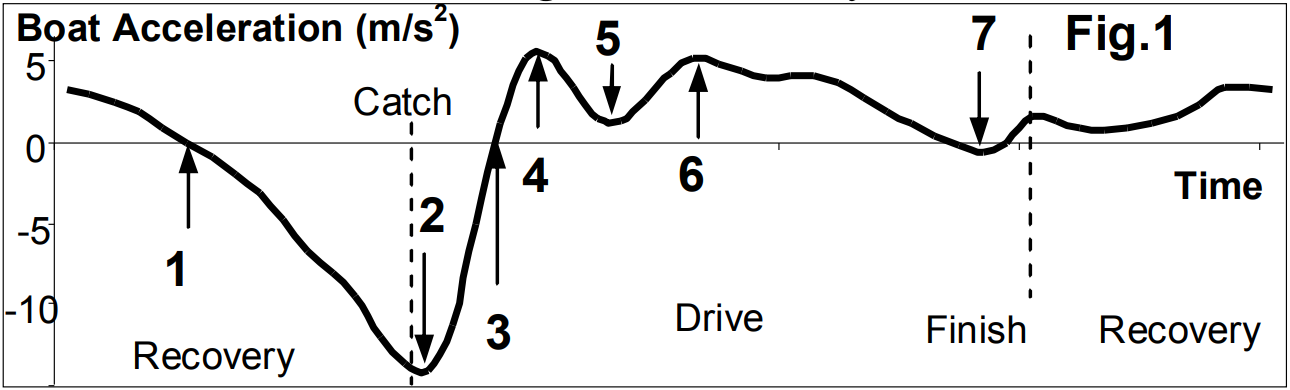
\includegraphics[width=0.7\textwidth]{rowing-stroke}
    \caption{Typical pattern of boat acceleration during the stroke cycle \cite{dr_valery_kleshnev_analysis_2012}}
    \label{fig:rowing-stroke}
\end{figure}

Rowing (and/or sculling) involves the propulsion of a racing shell \footnote{the long, light and narrow boat used for rowing} through the water, using either one or two oars. 
Rowing is cyclic and repetitive in its nature; every stroke is alike. 
The rowing stroke consists of two phases: the \textit{drive} and the \textit{recovery}. 
During the drive, the athelete pushes with their legs, moving towards the bow of the boat, with the oars in the water, thus accelerating the boat.
In the recovery, the athlete slides to the rear of the boat, while the boat slightly decelerates.
Figure \ref{fig:rowing-stroke} shows a typical acceleration pattern of a single stroke.

This acceleration pattern repeats with little fluctuation; thus one can determine the period with which it repeats and calculate the number of strokes being taken per minute. By combining this data with GPS readings, one can also calculate the distance the boat travels per stroke.

\chapter{Analysis}

\section{Identified issue}

A critical part of training is the \textbf{stroke rate}, which measures the number of strokes taken per minute of rowing. A higher stroke rate, with the same technique and power application, allows for more overall power to be applied per minute and thus move the boat faster. However, achieving a higher rate is difficult as the stroke length tends to shorten to compensate, especially as the rower fatigues. As such, many workout pieces are capped at a specified stroke rate, and it is necessary for the strokeman\footnote{the oarsman closest to the stern of the boat} and the cox\footnote{short for coxswain, the person steering the boat} to know the stroke rate of the boat and adapt the rowing stroke appropriately.

Another important part of training is the \textbf{split}, which measures the time taken, in minutes, to cover $500\si{\metre}$; in essence, it is the speed of the boat. 

\section{Existing solutions}

\subsection{Simple solution}

Average stroke rate can be measured by counting the number of strokes taken in a minute. All that is necessary is  a stopwatch. This is a simple solution, but it is not very accurate. Additionally, the coxswain should be focusing on steering, not counting strokes!

The split of the boat can be calculated by manually measuring the time taken to cover a known distance of water. This solution makes it difficult to account for steering line changes, and does not allow for realtime feedback of the boat's speed.

\subsection{Rowing stopwatches}

\begin{figure}[ht]
  \centering
  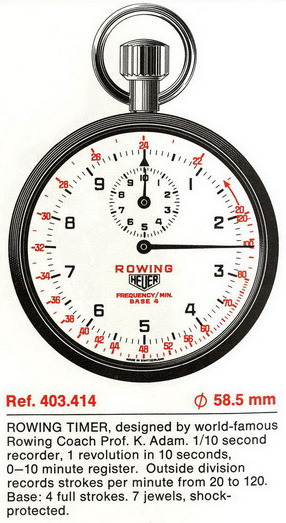
\includegraphics[width=0.3\textwidth]{rowing-stopwatch-heuer.jpg}
  \caption{A rowing stopwatch from the 1970-71 Heuer catalogue \cite{heuers_on_the_sea}}
  \label{fig:rowing-stopwatch-heuer}
\end{figure}

The 1960s saw the emergence of specialised mechanical rowing stopwatches. Figure \ref{fig:rowing-stopwatch-heuer} shows a rowing stopwatch manufactured by Heuer-Leonidas. These had a $1/10$th second resolution and were popular until the end of the 1980s.

\subsection{Nielsen-Kellerman StrokeCoach and SpeedCoach}

The first NK stroke rate meter was released in 1984, known as the Chronostroke. This was an electronic device that doubled as a stopwatch and allowed the cox or the coxswain to calculate the stroke rate. The 1990s saw the first PaceCoach, which coupled with inboard and outboard sensors such as an impeller to calcualte distance covered and real-time split.\cite{pacecoach}

The \href{https://nksports.com/speedcoach-gps-2}{NK SpeedCoach GPS (Model 2)} was released in 2012 and is a popular performance monitor for rowing on the water. 
It displays realtime information including split, stroke rate and the time and distance rowed. 
The first model used a physical magnet installed in the boat to record stroke rate, however, the second edition uses an inbuilt accelerometer for this and is completely wireless. 

An optional \textit{Training Pack} is available with Model 2 that adds software features such as Bluetooth support for heart rate monitor and synchronising training data to a smartphone.

The basic edition of the second model retails for \textsterling $399$; the \textit{Training Pack} is another \textsterling $99$.

Although the NK SpeedCoach is a popular rowing performance monitor, its price is certainly a barrier to entry. In addition, getting recorded data off the device is difficult, as Bluetooth connection is not reliable and requires synchronisation of \textit{all} the sessions on the stroke coach to obtain just the latest one.

\section{General solution statement}

The proposed solution, given the prevalence of smartphones in the modern world is a smartphone application that provides roughly equivalent core functionality to that of the commonplace NK SpeedCoach, including stroke rate, split and distance covered.

\section{Identified end user}

The end user is the coxswain or any of the rowers in the boat. In particular, the lower cost and availability of second-hand waterproof smartphones in comparison to the NK SpeedCoach would allow other rowers in the boat and not only the strokeman to be made aware of the rate. This solution would not be suitable for a coach in an adjacent boat, however, unlike a rowing stopwatch.

\section{Interviews}

\subsection{Interview with a coxswain}

An interview was conducted with the SPSBC 1st VIII cox, James Trotman. \\ His answers have been paraphrased.
\begin{enumerate}
  \item What do you look for in a stroke coach?
  
  If I was to buy a stroke coach I would want it to
  \begin{itemize}
    \item be \textbf{accurate} so that the stroke rate and splits can be acted upon in realtime,
    \item be \textbf{cheaper} than currently available products such as the NK SpeedCoach,
    \item be \textbf{easy to use} so that as much time as possible is dedicated to training,
    \item integrate with other existing software to simplify the post-session review process.
  \end{itemize}

  \item You are familiar with the NK SpeedCoach and use it in your daily outings. \\ Which of its metrics do you use?
  
  The NK SpeedCoach has a four-panel display, so usually I set it up to display a stopwatch, the stroke rate, split and distance covered. In a race I usually swap the distance covered for distance per stroke but even then I rarely use it [the distance per stroke metric]. As a cox I do not need to see my heart rate and so do not use this feature.
  
  \item Is there any functionality that you feel the NK SpeedCoach is lacking?
  
  You can export rowing sessions off the SpeedCoaches, but it is not a simple task. Their app is buggy and the Bluetooth connection between my phone and the SpeedCoach is not always reliable. Also the synchronisation process requires one to download \textit{all} the sessions off the SpeedCoach even if you are only interested in the latest one.

  This might be harder to implement, but it would also be amazing to have power curve analysis like on the \href{https://www.rp3rowing.co.uk/}{RP3} on the water, and perhaps other metrics such as check\footnote{the sudden dip in boat velocity at the point when the oar enters the water} or ratio\footnote{refers to the relationship between the amount of time spent on the drive and the recovery}.

  \item You have also examined the data produced by the \href{http://biorow.com/}{BioRow} in-boat telemetry system. \\ Which of those additional metrics provided by BioRow you found useful?
  
  We found the graph of boat acceleration somewhat useful, as we were told that our boat acceleration at the catch is too shallow. However, it was not made clear what the optimal shape of the graph should look like. The \textit{verticle angle + boat roll} metric once again indicated to us that the boat was not level during our session, but we could easily tell that this was the case even before the telemetry system was installed.

\end{enumerate}

\section{Specific solution statement}

A smartphone application is to be designed; one that will inform the user of the stroke rate and split and split of the boat in real time. Most people already have a smartphone with an accelerometer and a GPS sensor, which can be used to obtain data about the boat. In addition, since the tracking would be taking place on the phone itself, the need for synchronising sessions between a phone and a stroke coach would be eliminated.


\subsection{Practical considerations}

Although increasingly common, not many smartphones have a sufficient ingress protection rating to be comfortably taken into the boat. 
It is necessary to consider the requirement of a waterproof case, clamp or other holder that would allow the device to be affixed securely to the boat and prevent water damage in case of rain, waves or capsizing. 
One example would be a waterproof jogging armband: these are inexpensive, can be wrapped around a wing rigger \footnote{modern version of an \href{https://en.wikipedia.org/wiki/Outrigger}{outrigger} that spans across the middle from one saxboard to the other} and are a low barrier to entry.

\subsection{Specification}

A detailed specification is defined here that will be used to define the resulting application and the underlying technology.

The program \textbf{must}:
\begin{enumerate}
  \item be an application installable on any modern\footnote{released within the last five years} Android smartphone,
  \item require minimal configuration and interaction from the end user, and ideally none at all,
  \item display, in a realtime and an easy-to-read manner:
  \begin{itemize}
    \item the boat's stroke rate,
    \item the boat's split,
    \item the total distance rowed over the course of the session,
    \item the elapsed total session time
  \end{itemize}
  \item collect data during a rowing session using nothing but the hardware on the smartphone,
  \item provide start/stop functionality to record the rowing session for later review,
  \item allow the user to export the recorded rowing session as a \href{https://developer.garmin.com/fit/file-types/activity/}{\texttt{FIT} activity file} that can be imported into 3rd-party software, such as \href{https://strava.com}{Strava}, containing
  \begin{itemize}
    \item the geolocation of the boat,
    \item the speed of the boat,
    \item the cadence, or stroke rate, of the rowers,
    \item the estimated power generated by the rowers
  \end{itemize}
  \item be as battery-efficient as possible
\end{enumerate}

\chapter{Design}

\section{Input}

\subsection{Device hardware}

Almost all handheld Android smartphones have an accelerometer, since this is necessary for the screen auto-rotation feature, and many also feature either a gyroscope or a magnetometer.\cite{android_motion_sensors} 
The key component for this project is the accelerometer, however, the gyroscope and magnetometer could be used to improve the accuracy of the data.

The top $1822$ most popular Android devices on Geekbench, a popular benchmarking tool, have an average performance of $1018$, scoring slightly higher than a desktop Intel\textsuperscript{\textregistered} Core\texttrademark i$3$-$8100$ CPU. \cite{android_benchmarks} However, we cannot rely on such performance. If this application is to appeal to rowing clubs as a viable alternative to the NK SpeedCoach, it cannot require an equally-priced smartphone to run! Therefore the core features of this app must be optimised to perform well on lower-end devices.
Efficient algorithms reduce strain on the CPU and thus make the process more battery-efficient.

\section{Processing incoming data}

\subsection{Stroke rate}

As part of the Android software stack, a virtual sensor is available that filters out acceleration due to gravity from the raw signal produced by the accelerometer.\cite{android_linear_accel} 

The acceleration and linear acceleration sensors output a vector with $x$, $y$ and $z$ axes, which are oriented relative to the device, with the $z$-axis coming out of the screen of the device. 
Since the boat is travelling linearly and we do not need an accurate numeric value for the accleration, it is enough to calculate the magnitude of the linear acceleration
\[
  \abs{\textbf{a}} = \sqrt{x^2 + y^2 + z^2} 
\] 
to obtain a repeating (with slight variation) pattern. Since we are taking the magnitude, the phone can be placed in any orientation and stroke rate detection can still be performed. Or, if the phone for example slips or changes position during the rowing session, stroke rate detection would not be interrupted. 

The shape of the acceleration readings produced by the above equation should are assumed to be similar in pattern to the absolute value of the acceleration pattern shown in in figure \ref{fig:rowing-stroke}.

To calculate the stroke rate from the acceleration pattern, a Fourier transform is proposed. The Fourier transform is a discrete transform that can be used to calculate the frequency of a signal. It works by decomposing the sampled repeating pattern into a series of sinusoids. The frequency of the sinusoid with the greatest amplitude is selected as the true stroke rate. More specifically, a Sliding Discrete Fourier Transform (\textit{SDFT}) can be employed. It is an efficient ($O(n)$) algorithm that can be used to calculate the frequency of a signal.

\begin{displayquote}
  The sliding DFT is a recursive algorithm to compute successive Fourier transforms of input data frames that are a single sample apart.\cite{sliding_smoother_than_jumping} 
\end{displayquote}

Although the SDFT is an efficient algorithm, it is nonetheless rather calculation-heavy. Stroke rate calculation ought to be performed on a separate thread to not slow down the graphical user interface.

\subsection{Programming languages and frameworks}

There are three primary supported programming languages for developing Android apps: C++, Java and Kotlin. Kotlin is a modern statically typed programming language used by over 60\% of professional Android developers. It is selected for this project due to the following advantages: 
\begin{itemize}
  \item Kotlin is cross-compatible with Java code, so although the language is relatively new, any libraries and frameworks developed for Java will work with Kotlin.
  \item Kotlin has many modern language features that draw inspiration from functional programming and allow for more concise code.
  \item Kotlin's coroutine functionality makes asynchronous programming simple and more efficient.
  \item Kotlin makes handling nullability of variables and objects far easier, to help avoid Java's dreaded \texttt{NullPointerException}. 
\end{itemize}


\chapter{Technical solution}

\section{Data collection}

\section{Data processing}

\subsection{SlidingDFT.kt}

As specified in the design stage, the incoming acceleration readings are to undergo a Sliding Discrete Fourier Transform (SDFT) to find the dominant frequency.

\begin{displayquote}[\cite{sliding_smoother_than_jumping}]
  That means that in order to forget the oldest sample and accept a new sample, all that is needed is for the $n$th frequency amplitude is an addition, a subtraction and a complex rotation by $2\pi n / N$ radians. As we know that the samples are real this is a little simpler than it might appear.

  There remains the problem of starting, but if we assume that the signal was silent until the first sample, then the transform is also zero and so we can slide the samples in one at a time without creating an initial FFT [Fast Fourier Transform].
\end{displayquote}

\begin{figure}[h!]
  \centering
  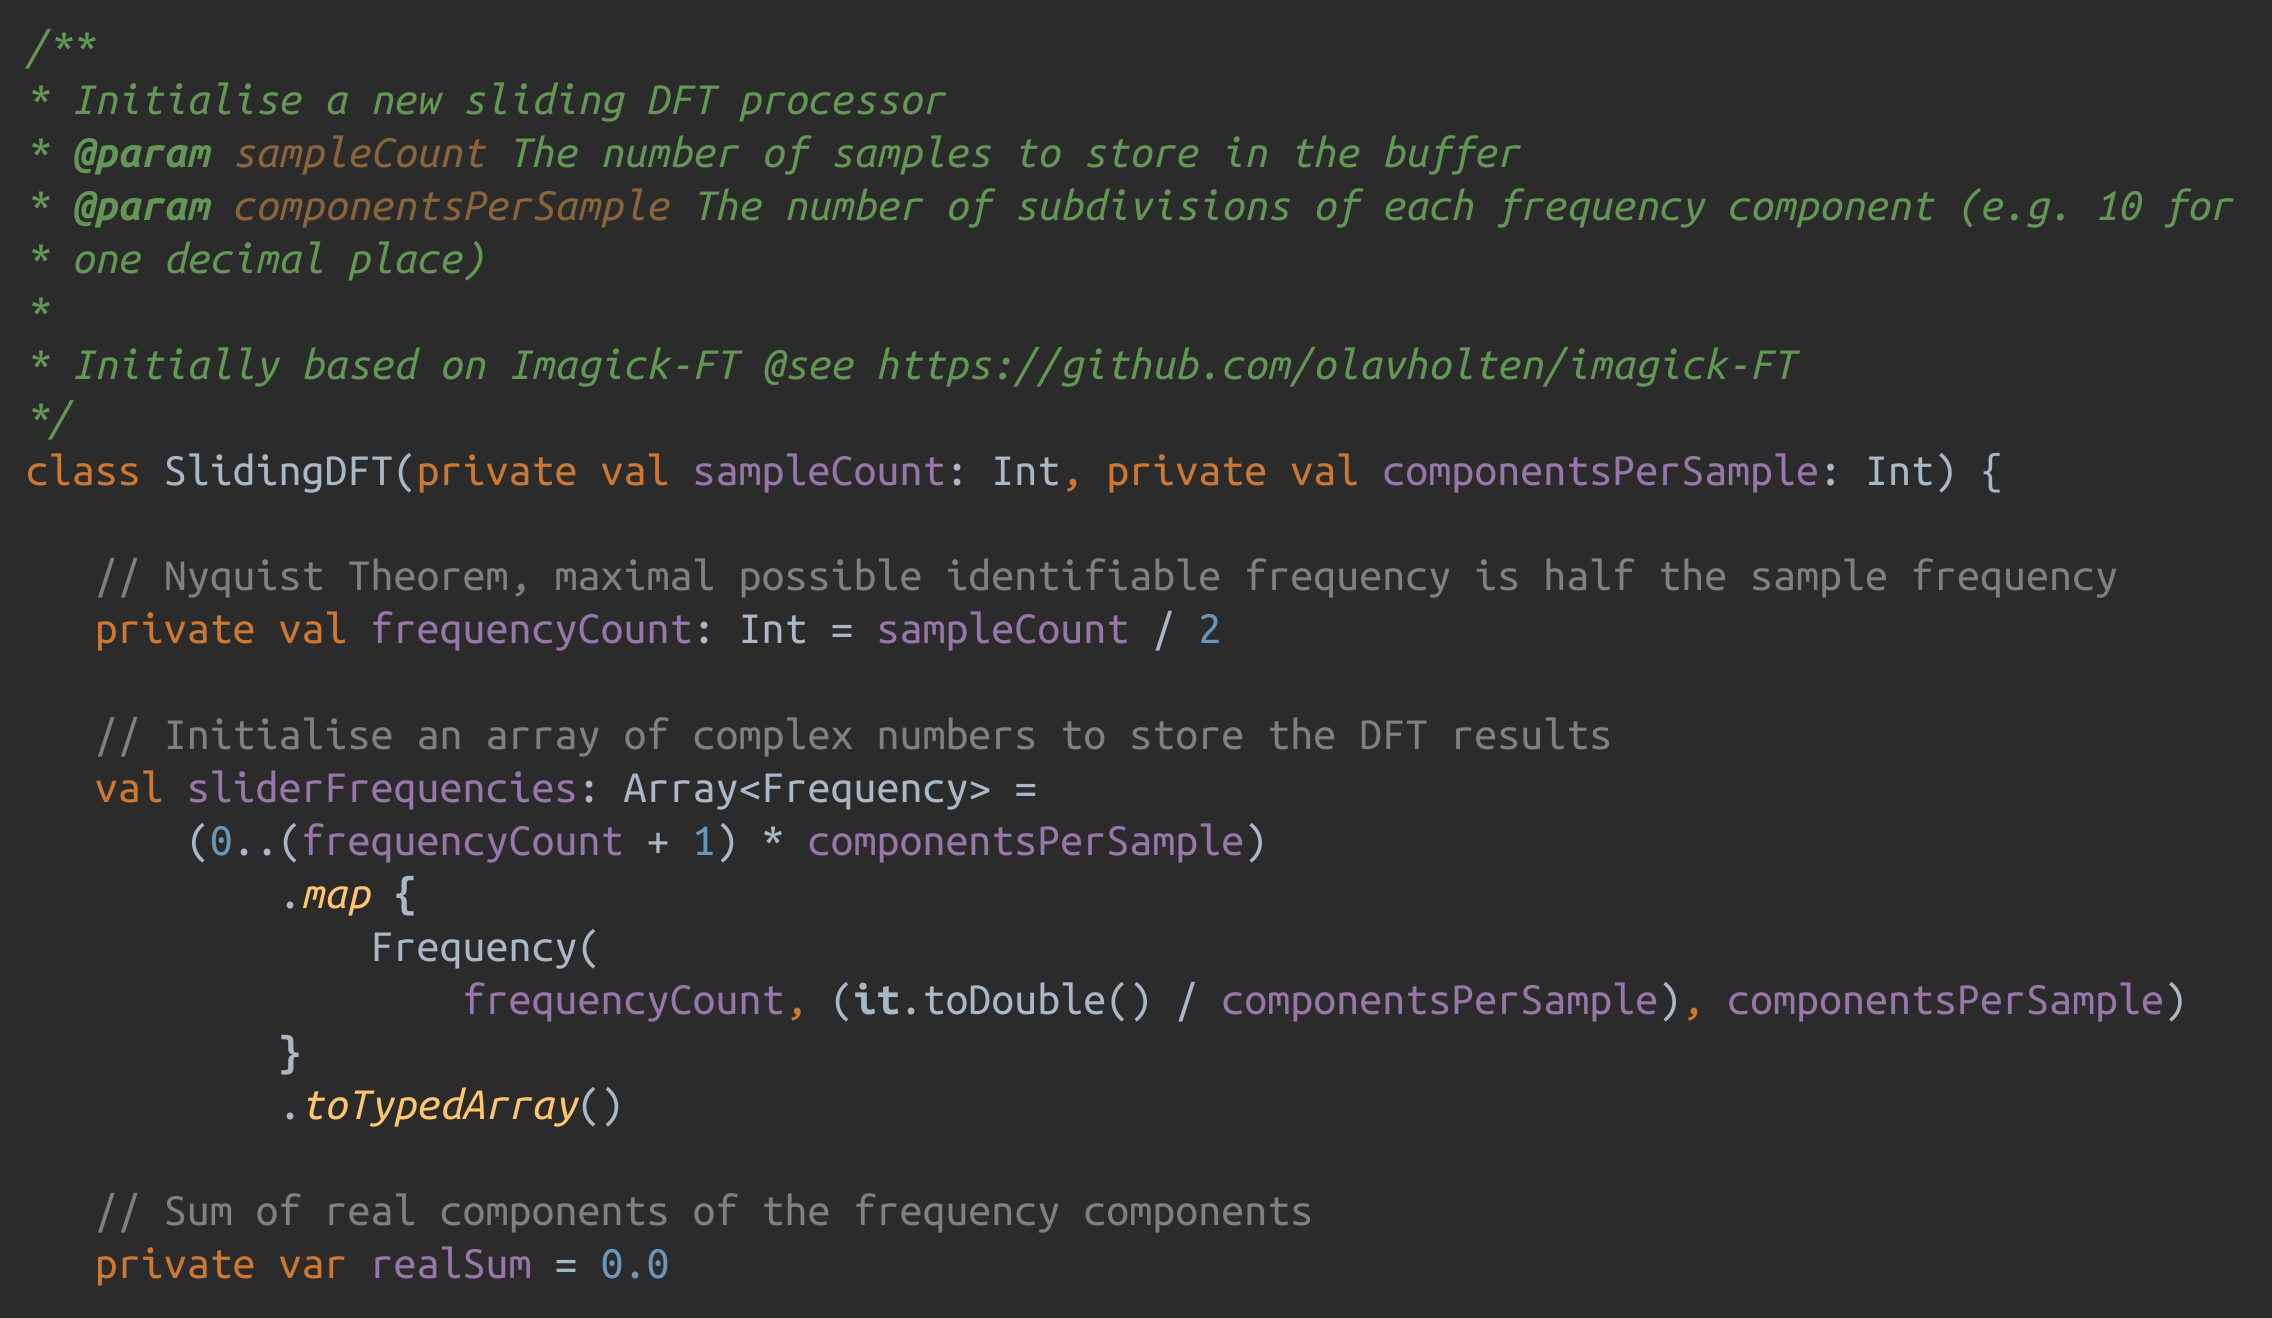
\includegraphics[width=1.0\textwidth]{code-slidingDFT.png}
  \caption{}
  \label{fig:slidingDFT}
\end{figure}

The \texttt{SlidingDFT} class is initialised with the number of successive samples to be used. The constructor and initialisation code is shown in figure \ref{fig:slidingDFT}. The maximal possible identifiable frequency is half the sample frequency according to Nyquist's theoreom, so this is used to determine the number of frequency bins available. A later addition also includes a \texttt{componentsPerSample} parameter that allows for one to subdivide the frequency bins into a number of sub-bins to allow for greater frequency resolution. A DC\footnote{DC for direct current, the frequency bin for the zero-frequency sinusoid} and Nyquist\footnote{the frequency bin for the maximal frequency} bin are also included, so the number of available frequency bins is $\frac{N}{2} + 2$.

\begin{figure}[h!]
  \centering
  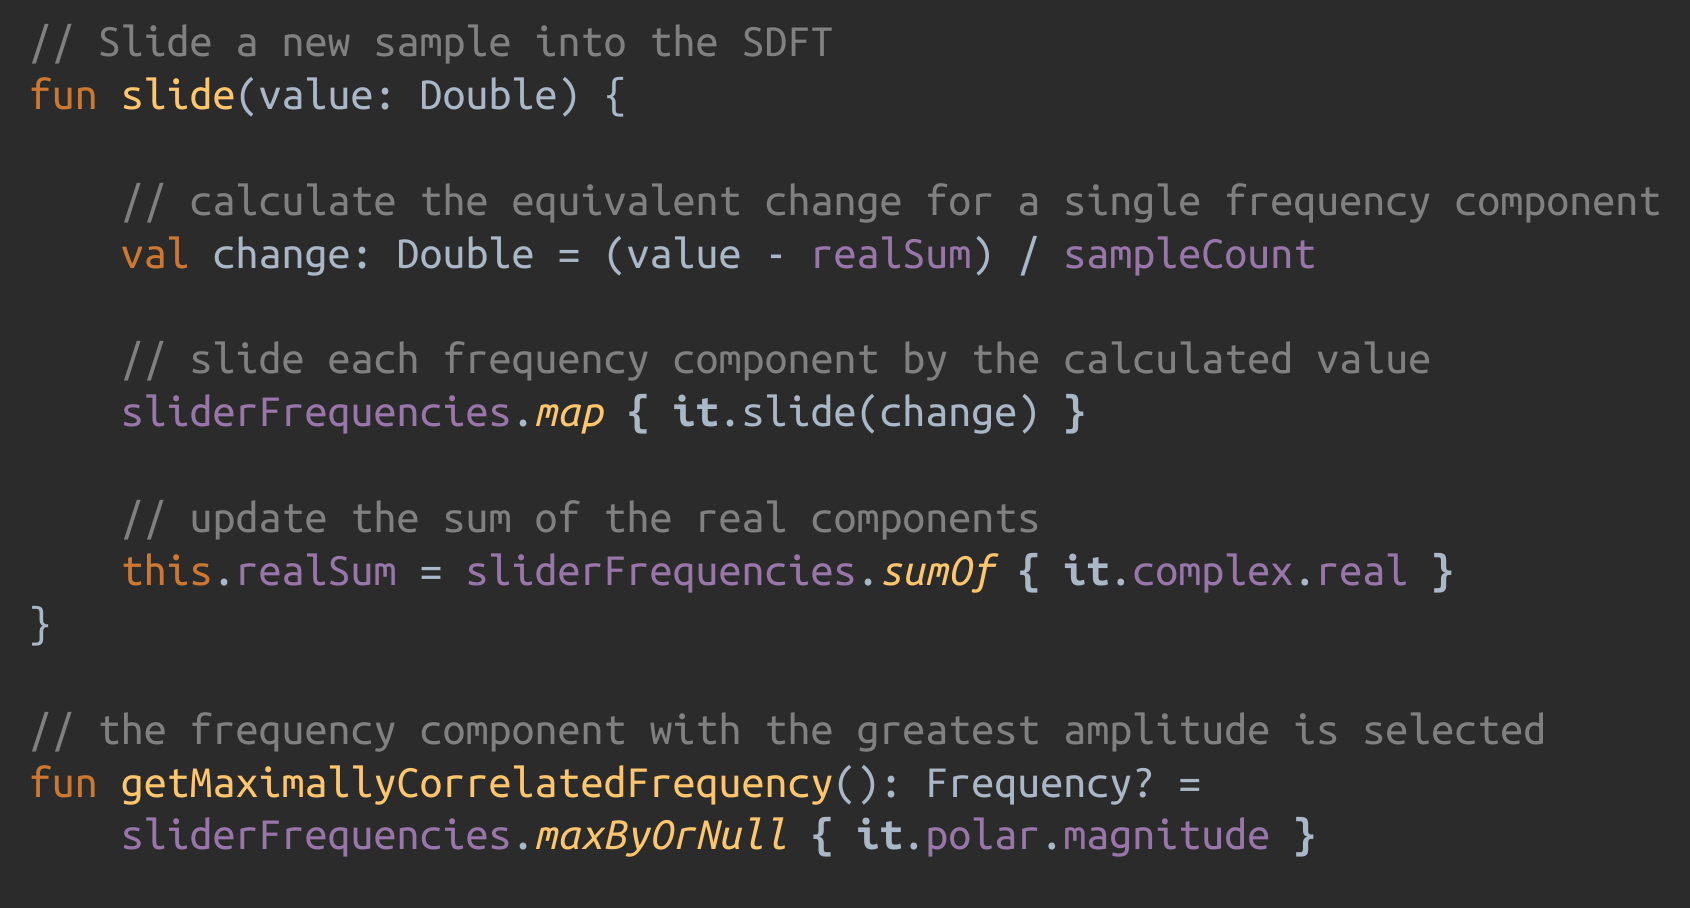
\includegraphics[width=1.0\textwidth]{code-SDFT-slide.png}
  \caption{}
  \label{fig:slideBest}
\end{figure}

The sum of the real components of all the frequency bins is stored and recalculated on each addition of a new sample. This is also used to calculate the equivalent per-bin shift in value given the newly slid-in reading. The calculated shift in value is applied to each frequency bin in turn. A function is also  provided to calculate the dominant frequency at the given moment in time -- it returns the wavelength of the frequency bin with the greatest magnitude. The code for the two aforementioned methods is shown in figure \ref{fig:slideBest}.

Within the \texttt{SlidingDFT} class an inner class called \texttt{Frequency} is defined, the code for which is displayed in figure \ref{fig:innerClassFrequency}. This class represents a single frequency component of the SDFT. As stated in the paper, each frequency component experiences a rotation of $2\pi n / N$ radians, where $n$ is the wavelength and $N$ is the window size. Since we halved the window size to obtain the total number of frequency bins, the factor of $2$ cancels out. A correction is applied for DC and Nyquist frequency bins.

\begin{figure}[h!]
  \centering
  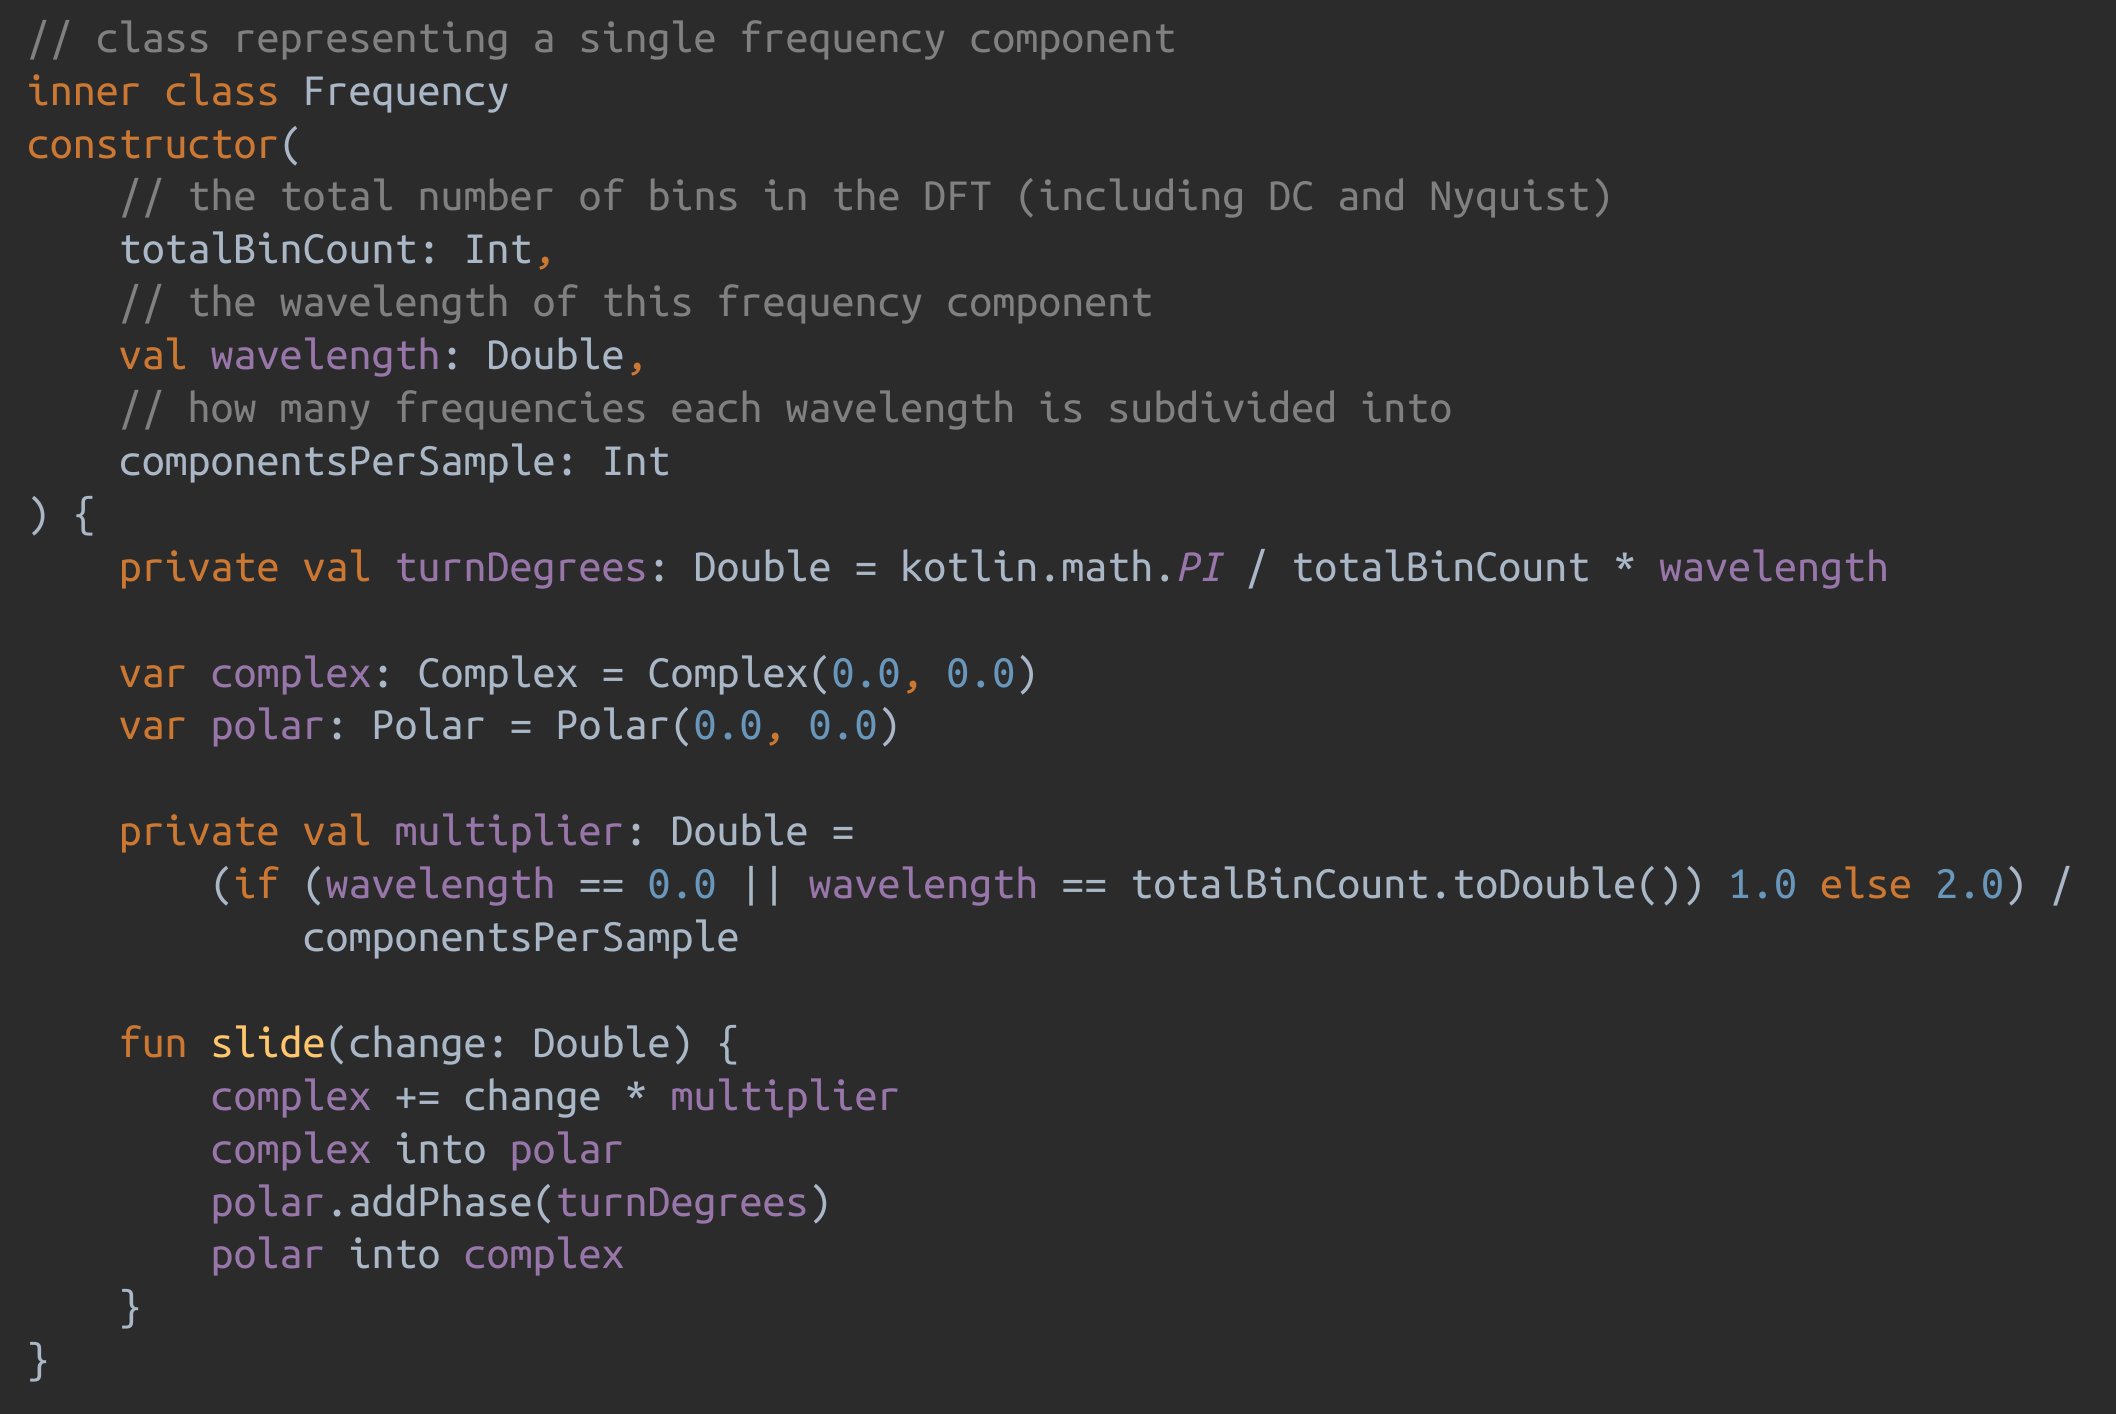
\includegraphics[width=1.0\textwidth]{code-innerClassFrequency.png}
  \caption{}
  \label{fig:innerClassFrequency}
\end{figure}

\texttt{Polar} and \texttt{Complex} are two data classes that represent a complex number in different forms. The two of them make use of a feature of Kotlin that I find rather appealing: infix functions. Both have an \texttt{into} function that converts the imaginary number from one representation into another. By using these \texttt{into} methods, we avoid recreating the objects when the imaginary number is changed from one representation to another in the \texttt{slide} function of the inner \texttt{Frequency} class, making the algorithm more efficient.

\begin{figure}[h!]
  \centering
  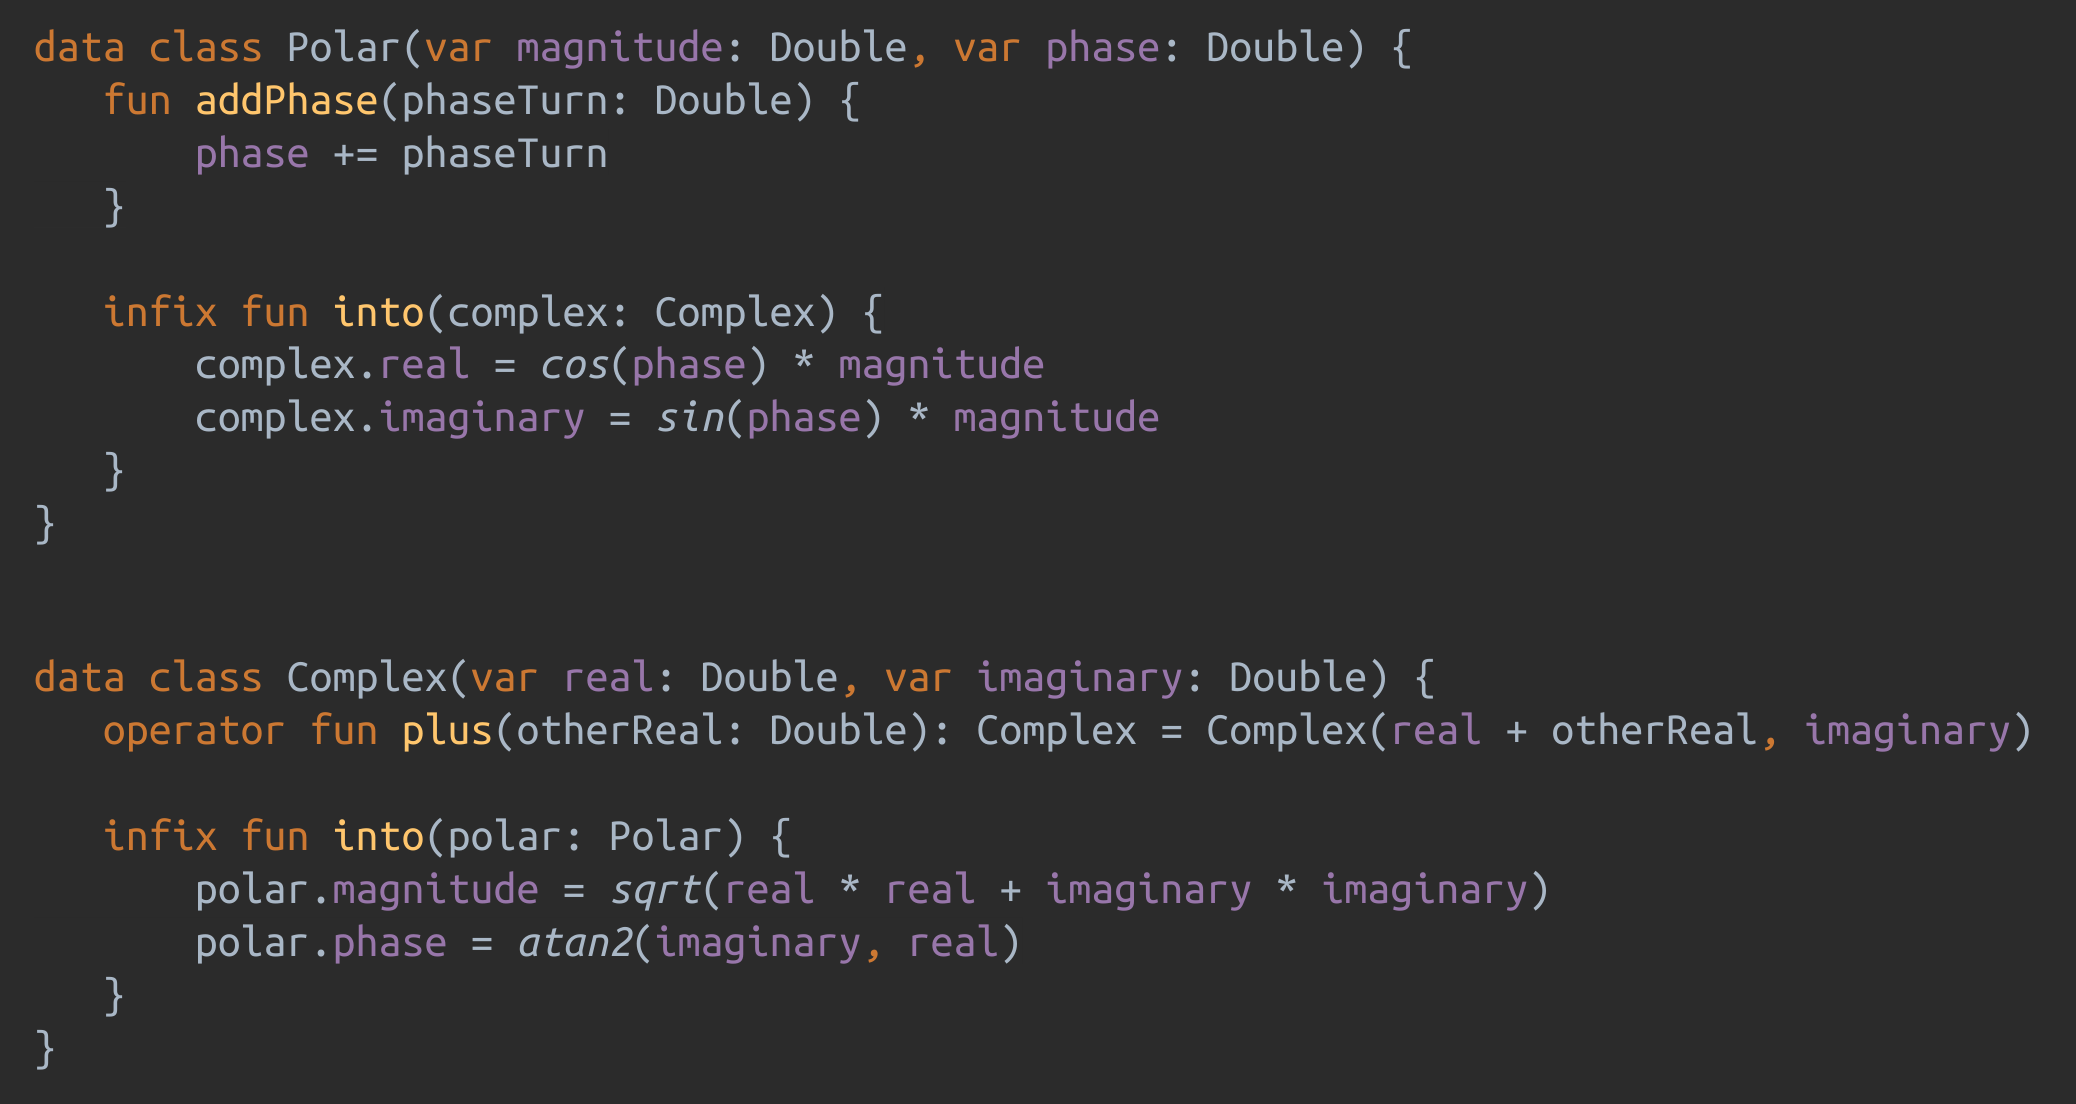
\includegraphics[width=1.0\textwidth]{code-SDFT-complex-polar.png}
  \caption{}
  \label{fig:complexPolar}
\end{figure}

Unfortunately in testing the sliding DFT proved to be inadequate for the task at hand. Although incredibly efficient (the most costly operation being the calculation of a sine and cosine) it was not able to accurately calculate the frequency of the signal. It was discovered only after some head-bashing firmly within the implementation stage that a fundamental downside of the Discrete Fourier Transform is that it is not possible to do DFT with low latency and fine frequency resolution at low frequencies.\cite{dsp_stack_dft} The frequency resolution is limited by the sampling rate, which, for a modern smartphone is somewhere in the region of 50Hz. This is insufficient to find a reasonable compromise.

By adding more frequency bins, a far higher resolution is achieved, with accuracy as far as one decimal place for the stroke rate. The downside to this is an incredibly increase in latency, with stroke rate persisting for up to half a minute (!) after device movement has ceased. Since the limiting factor is the sampling frequency, this would be a possible solution. And, with careful handling, a \texttt{SensorDirectChannel} can be accessed on Android that provides sensor sampling frequencies in excess of 500Hz, more than ten times as frequent as the smartphone's native sampling rate. However, this significantly increases power consumption for the device, both due to the increased accelerometer sampling rate and due to the increased overhead for processing more samples per second as well as the memory that would be required to store an adequately sized buffer for the readings.

As such, it was time to return back to the drawing board and a new solution was proposed.


\subsection{Autocorrelator.kt}

The \texttt{Autocorrelator} class provides utility methods for scoring the input readings according to their autocorrelation.

\subsubsection{\texttt{getFrequencyScores(data)}}

The method shown in figure \ref{fig:getFrequencyScores} slides a copy of the second half of the data over itself, scoring each offset with the correlation of the slid data and the previous signal.

The discrete autocorrelation $R$ at lag $\tau$ for a discrete time signal $X$ is given by
\begin{equation*}
  R(\tau) = \text{Corr}\left(X_n,\,X_{n-\tau}\right)
\end{equation*}
Correlation of two data sets $X$ and $Y$ is given by the below formula (from the Further Maths syllabus!)
\begin{equation*}
  \text{Corr}\left(X, Y\right) = \frac{\text{Cov}\left[X, Y\right]}{\sqrt{\text{Var}\left(X\right)\text{Var}\left(Y\right)}}
\end{equation*}
Since in this case $X$ and $Y$ are the same underlying data, except with different lag, their variances must be the same. The denominator can be simplified to $\text{Var}\left(X\right)$.

Expressing the covariance and variance as a summation, the below formula is obtained, where $\mu$ is the mean of the data.
\begin{equation}
  \frac{\sum \left(X_i - \mu\right)\left(X_{i-\tau} - \mu\right)}{\sum \left(X_i - \mu\right)^2}
\end{equation}

\begin{figure}[h!]
  \centering
  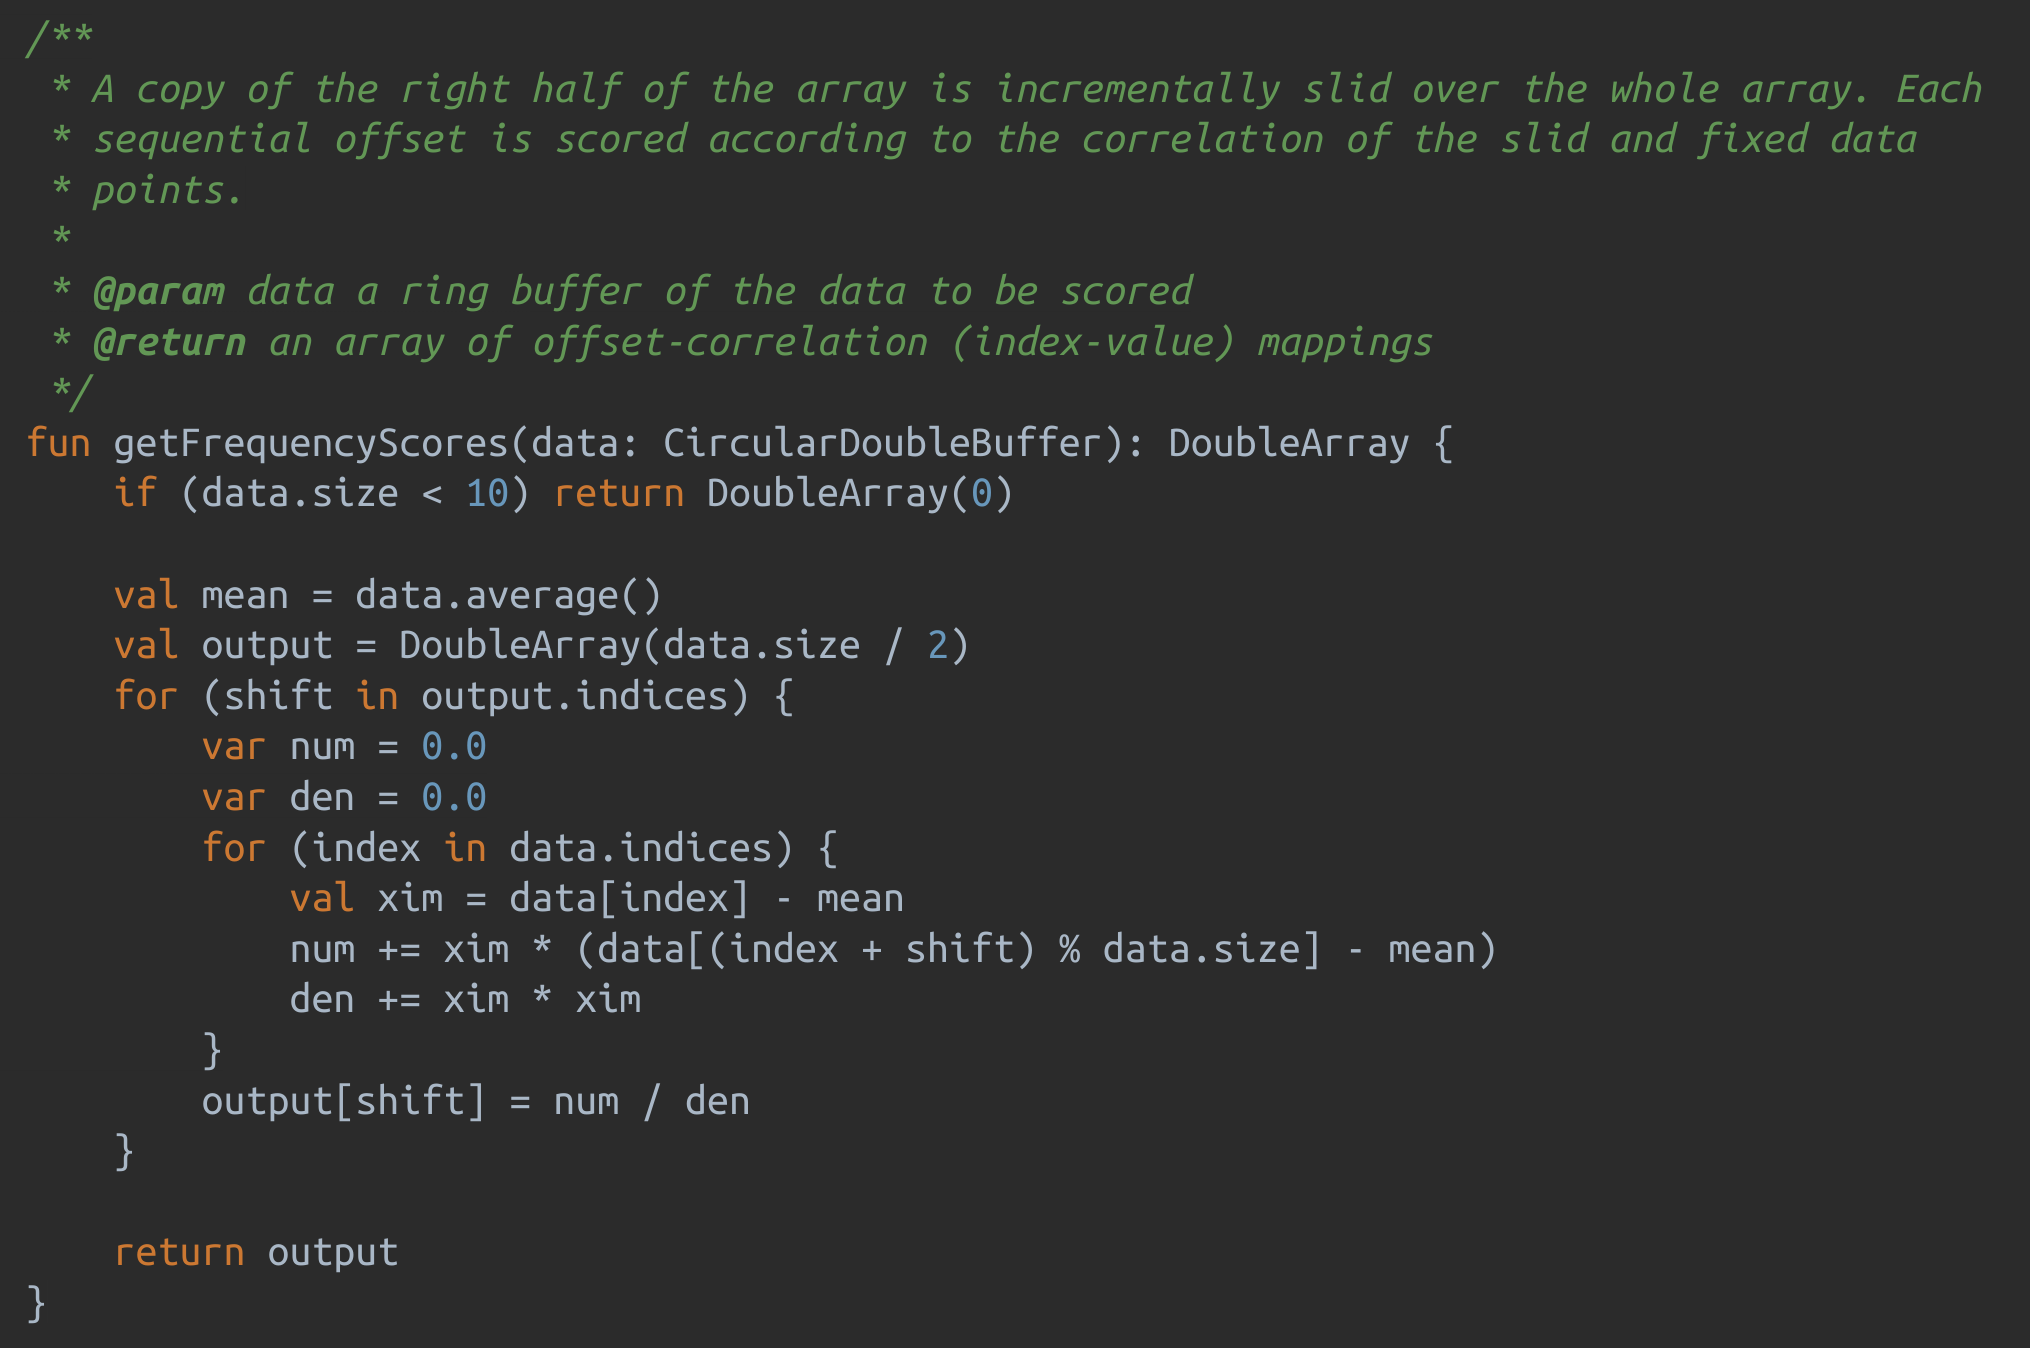
\includegraphics[width=1.0\textwidth]{code-autocorrelator-getFrequencyScores.png}
  \caption{}
  \label{fig:getFrequencyScores}
\end{figure}

The mean is calculated using an inbuilt method provided by Kotlin's \texttt{Collection} interface.
There are $\frac{N}{2}$ possible lag values, where $N$ is the number of data points in the ring buffer.
The correlation scores are calculated for each lag, or offset, and saved into a \texttt{DoubleArray}. The \texttt{DoubleArray}'s index represents the lag, which is recorded as a number of samples, and the value is the calculated correlation for this offset. This method assumes that the sampling rate remains fairly constant for its results to be reliable, and this is the case for any decent accelerometer.


\subsubsection{\texttt{getBestFrequency(correlations)}}

\begin{figure}[h!]
  \centering
  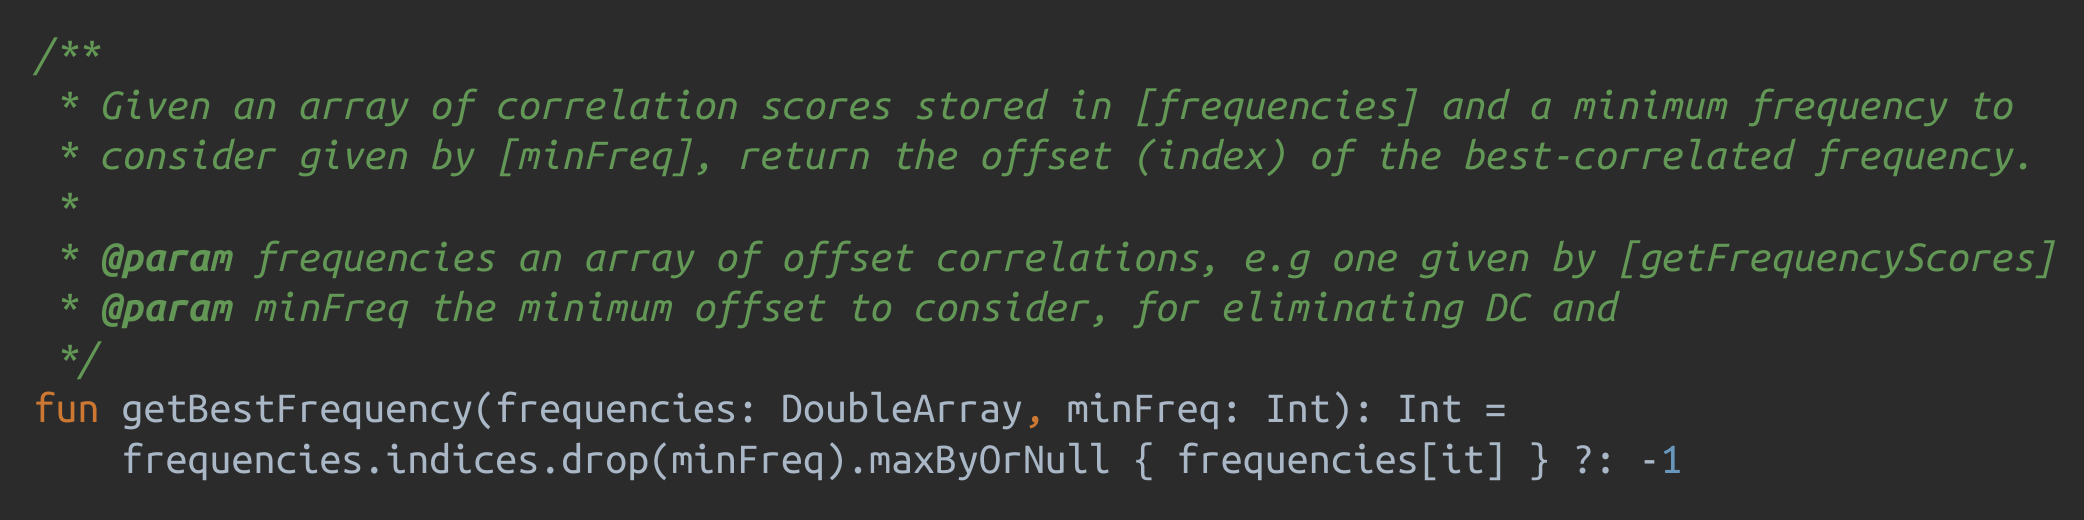
\includegraphics[width=1.0\textwidth]{code-autocorrelator-getBestFrequency.png}
  \caption{}
  \label{fig:getBestFrequency}
\end{figure}

The method shown in \ref{fig:getBestFrequency} selects the "best" frequency out of the provided autocorrelation array by choosing the one with the highest value. Stroke rates below a specified threshold are ignored. This is because, naturally, a tiny offset (e.g. $1$ sample) will produce a near-perfect correlation. Since very low-rate stroke detection is not necessary these frequencies can be discounted.

\subsection{\texttt{CircularDoubleBuffer.kt}}

The \texttt{CircularDoubleBuffer} class provides an implementation of a circular buffer, also known as a ring buffer, for storing \texttt{Double} values. Its primary use in the context of this application is for storing recent acceleration readings. A circular buffer was chosen for its memory efficiency and fast append operations. It fulfills the obligations of Kotlin's \texttt{Collection} interface.

\begin{figure}[h!]
  \centering
  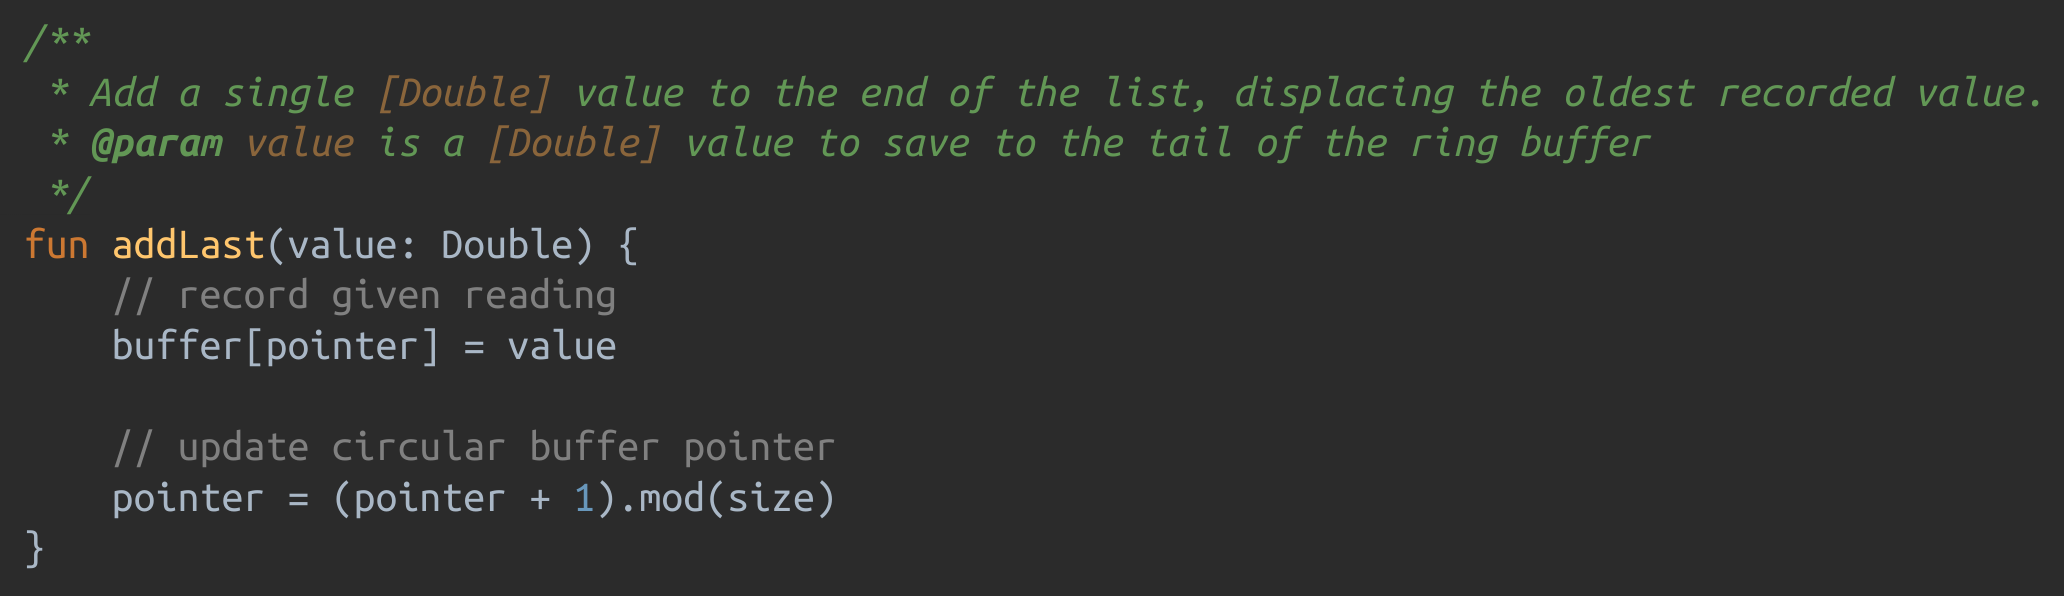
\includegraphics[width=1.0\textwidth]{code-CircularDoubleBuffer-addLast.png}
  \caption{}
  \label{fig:addLast}
\end{figure}

A single append method is necessary: \texttt{addLast(double: Double)}, the code for which is shown in figure \ref{fig:addLast}. This function stores the new value at the rear of the buffer, thus displacing (overwriting) the oldest value in the list which is no longer necessary for consideration. 

The \texttt{pointer} variable always points to the next slot to be filled, so it is incremented only after the value has been stored. The Kotlin \texttt{mod} operator is used as opposed to the infix \texttt{\%} operator, which is shorthand for \texttt{rem}. This is due to a subtlety in their functionality. The \texttt{mod} operator will always, as in mathematical modular arithmetic, return a value between $0$ and $n-1$, where $n$ is the value with respect to which modulo is taken. On the other hand, the \texttt{rem} operator can return negative values which could crash the application if it tries to access a negative index in the underlying \texttt{DoubleArray}.

\begin{figure}[h!]
  \centering
  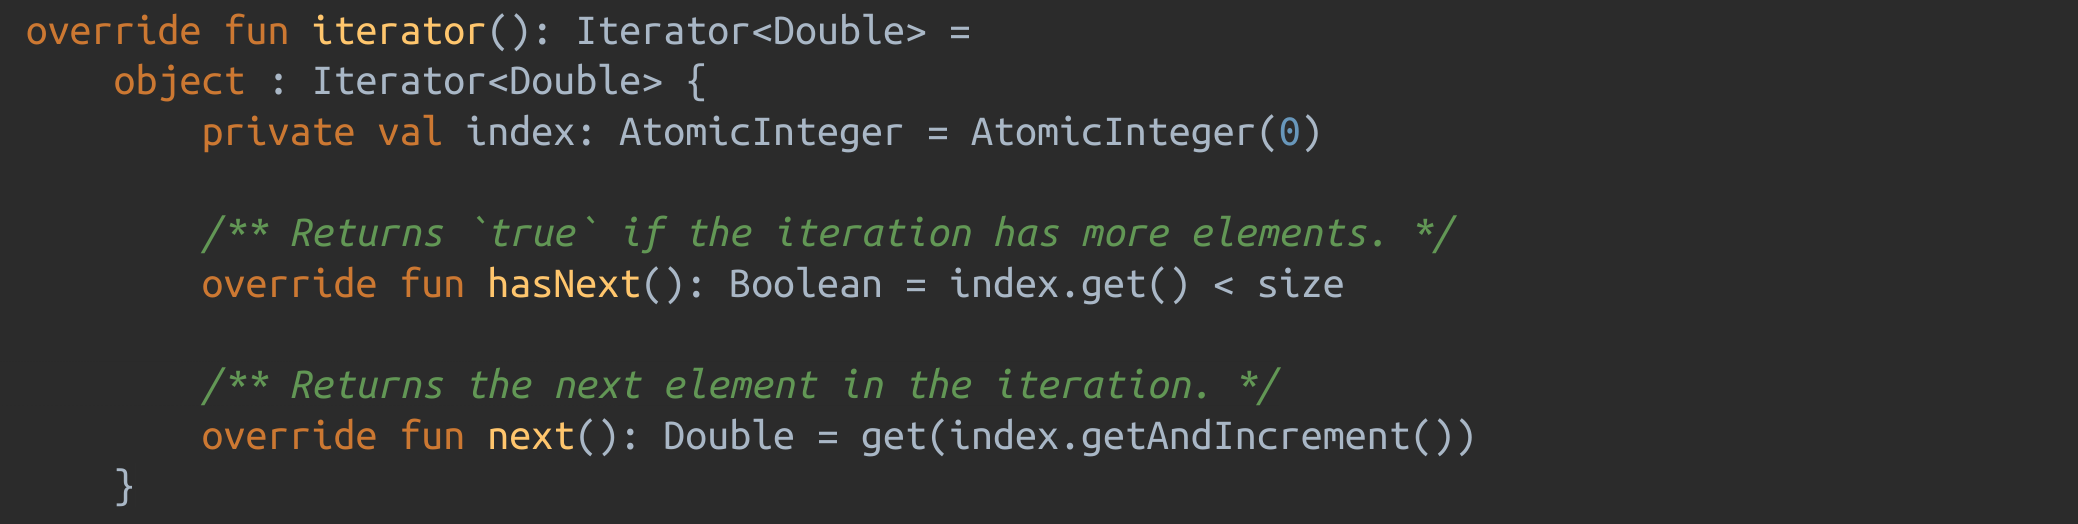
\includegraphics[width=1.0\textwidth]{code-CircularDoubleBuffer-iterator.png}
  \caption{}
  \label{fig:iterator}
\end{figure}

In addition, the \texttt{CircularDoubleBuffer} overrides the \texttt{iterator()} function of the parent \texttt{Collection} interface, as shown in figure \ref{fig:iterator}. This allows programs that use the \texttt{CircularDoubleBuffer} to iterate through the its elements as any other list in Kotlin with the \texttt{for (element in circularDoubleBuffer) \{ ... \}} syntax. 

An \texttt{AtomicInteger} was used instead of the normal \texttt{Int} class for thread-safe operations in a multithreaded context. This allows the \texttt{CircularDoubleBuffer} to be used from separate parts of the application without concern for concurrent access exceptions.

\subsection{\texttt{DataProcessor.kt}}

The \texttt{DataProcessor} class handles the processing of incoming acceleration and location data. Accelerometer readings are smoothed and stroke rate is calculated; it tracks the total distance travelled over the course of the rowing session and informs any UI listeners of updates of any of the aforementioned metrics through callbacks. It is also responsible for persisting the calculated stroke rate, speed, and other characteristics to the application database.

The processing of the data is a computationally expensive process; since it would be unfavourable to slow down the user interface, most of the functionality of \texttt{DataProcessor} is executed on another thread. Instead of launching a full-on separate thread, we can use a functionality built into Kotlin called coroutines. 

The Kotlin team defines coroutines as "lightweight threads". They are in essence tasks that can be executed by an actual thread. Kotlin coroutine jobs can be paused and resumed, passed between different actual threads and allow for easy handling of asynchronous execution. The context of the coroutine includes a coroutine dispatcher that determines what thread the corresponding coroutine uses for its execution.\cite{kotlin_dispatchers}

\begin{figure}[h!]
  \centering
  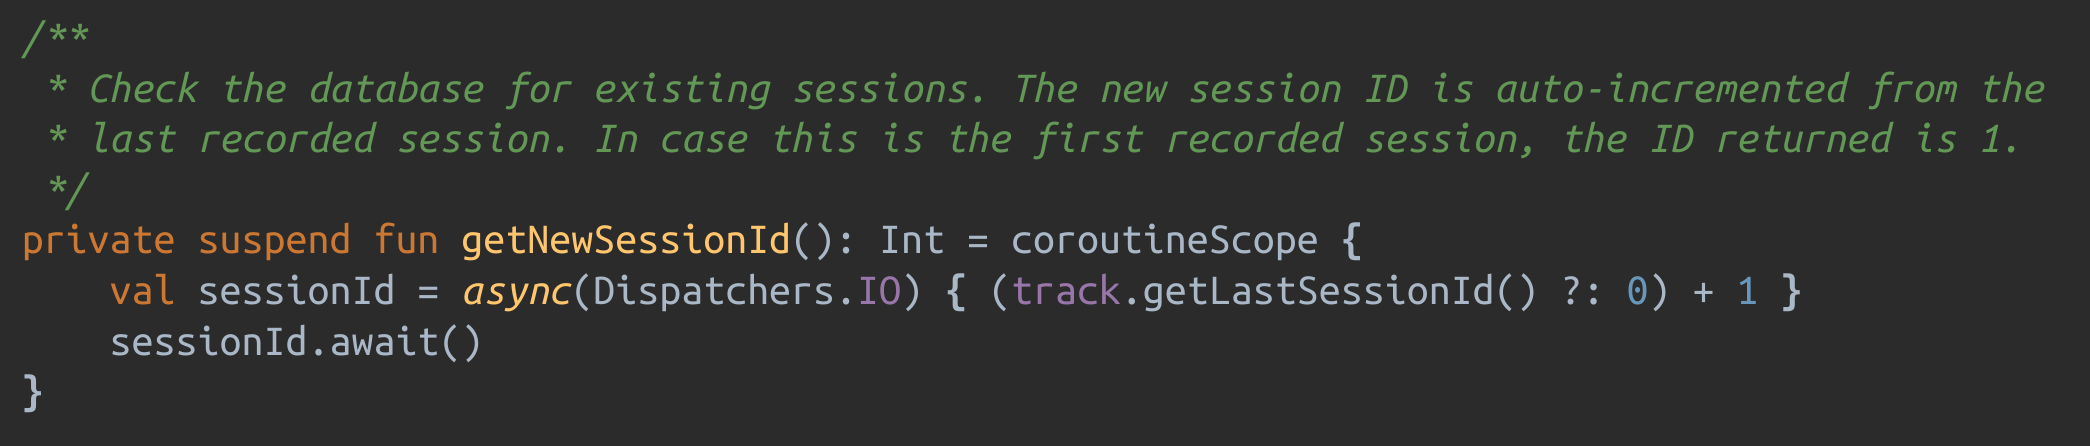
\includegraphics[width=1.0\textwidth]{code-dataProcessor-getSessionId.png}
  \caption{}
  \label{fig:dataProcessorGetSessionId}
\end{figure}

For example, the \texttt{getNewSessionId} function shown in figure \ref{fig:dataProcessorGetSessionId} gets the next sequentially availabe session ID. \texttt{Dispatchers.IO} is passed as an argument to the \texttt{async} function to specify that this command should be run on the applications I/O thread, as this function requires a SQL database query.

\begin{figure}[h!]
  \centering
  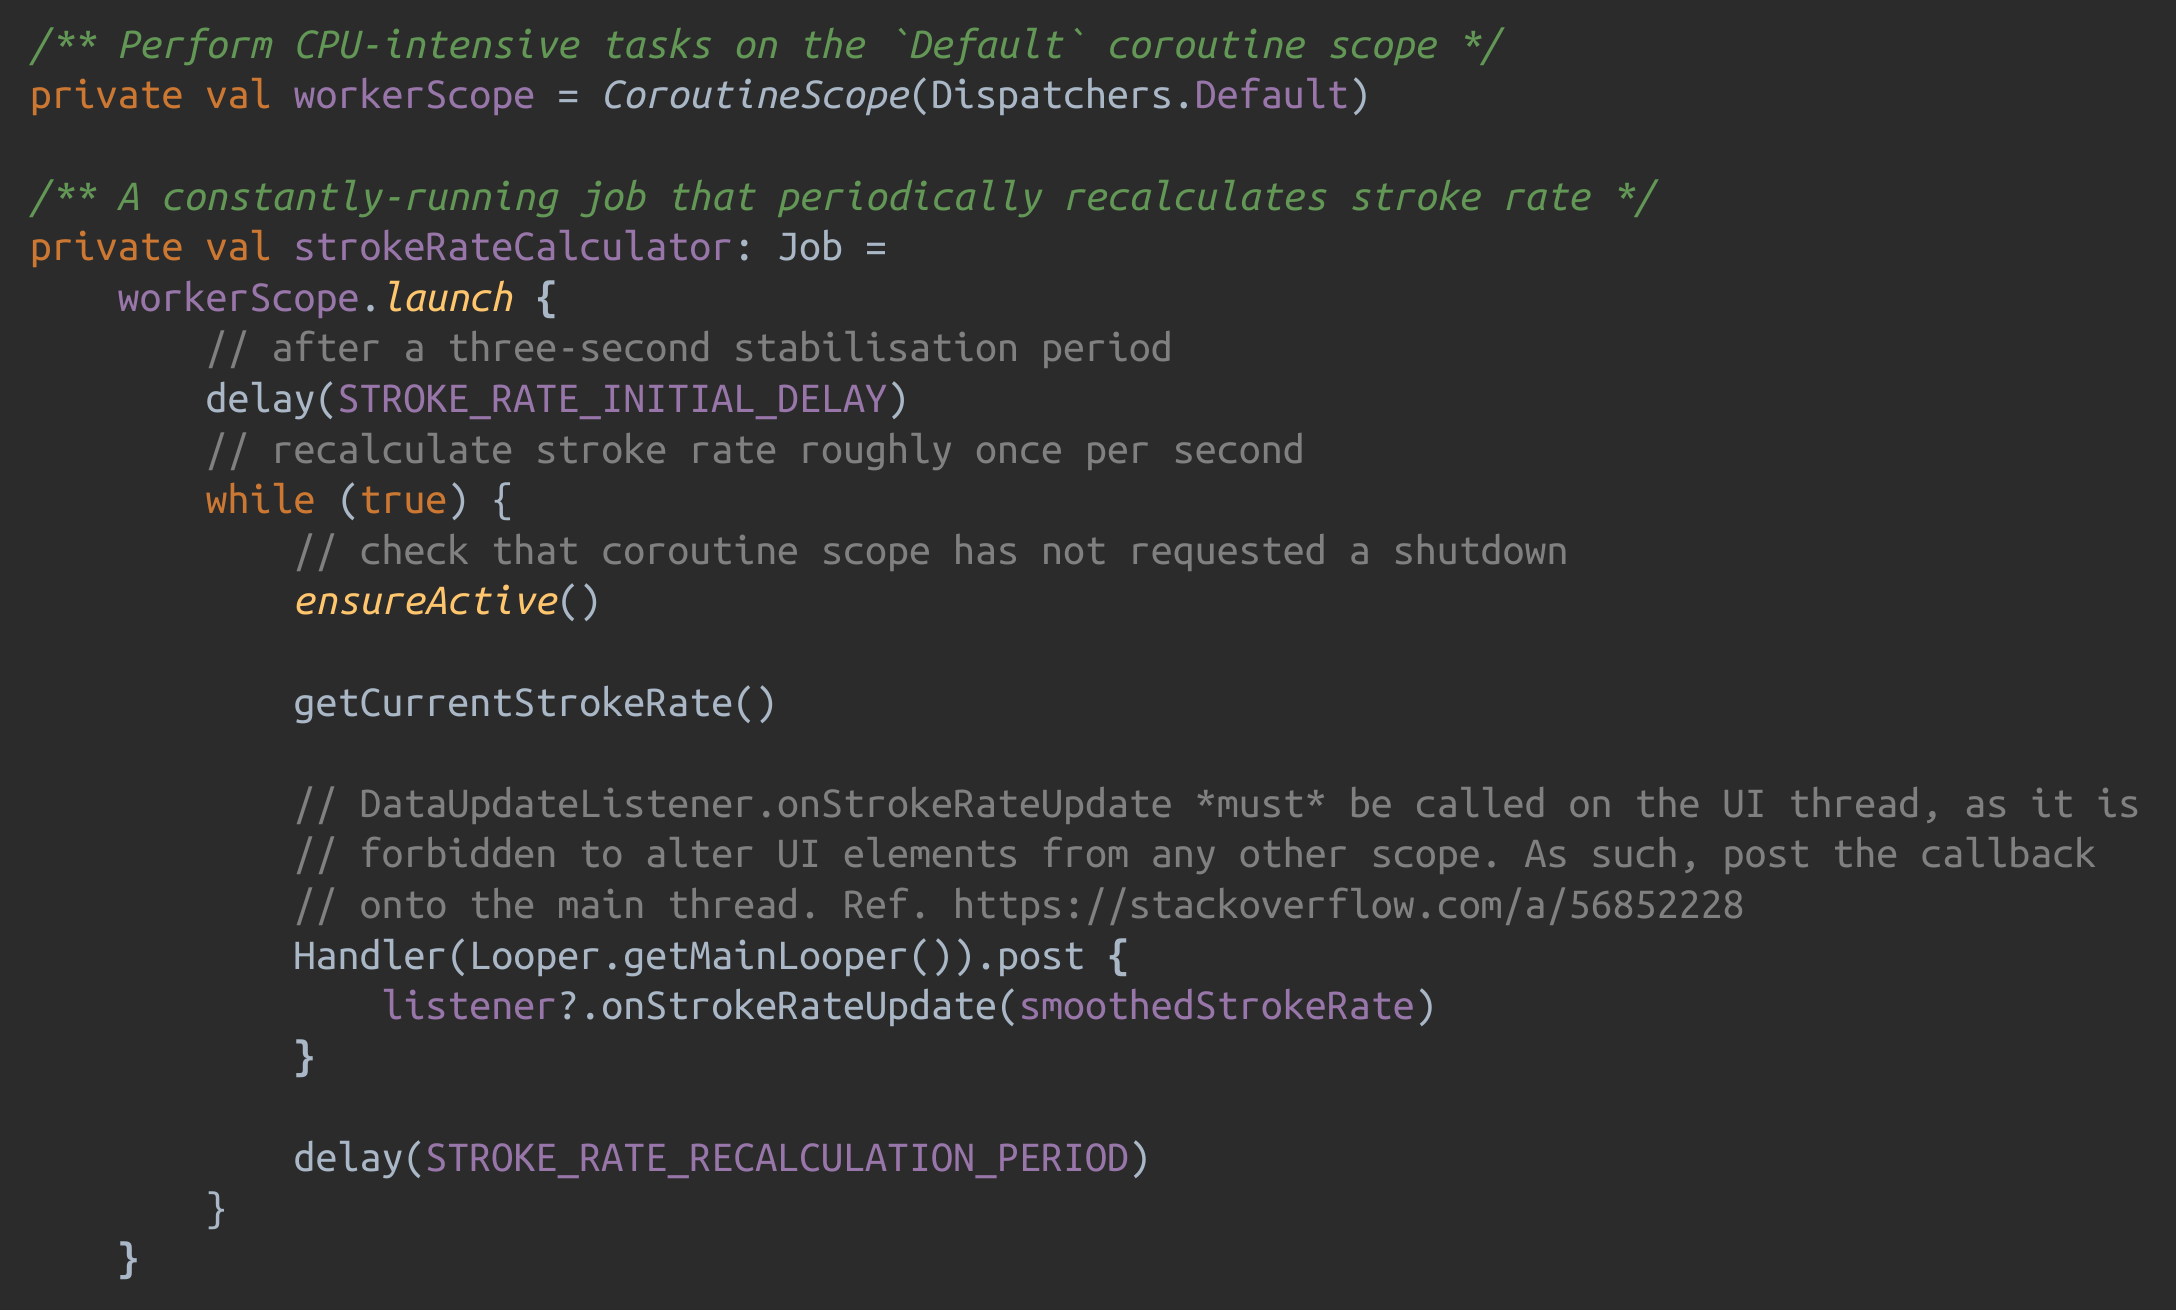
\includegraphics[width=1.0\textwidth]{code-dataProcessor-strokeRateCalculator.png}
  \caption{}
  \label{fig:strokeRateCalculator}
\end{figure}

The stroke rate is calculated by an infinitely-running coroutine job that executes on the \texttt{Default} coroutine scope, i.e. a worker non-UI thread. The code for this task is shown in figure \ref{fig:strokeRateCalculator}. 

A call to the coroutine-provided function \texttt{ensureActive} checks that the associated coroutine scope is still being used. This way, if an unhandled exception is encountered on the main thread this infinite job would still terminate despite no explicit call to do so.

However, since the stroke rate is being calculated in a worker scope, the callback to inform the listener of an updated stroke rate value has to be posted to the main thread before it can be executed. This is because Android UI elements are protected in that they cannot be modified by code running on anything but the main UI thread.

\begin{figure}[h!]
  \centering
  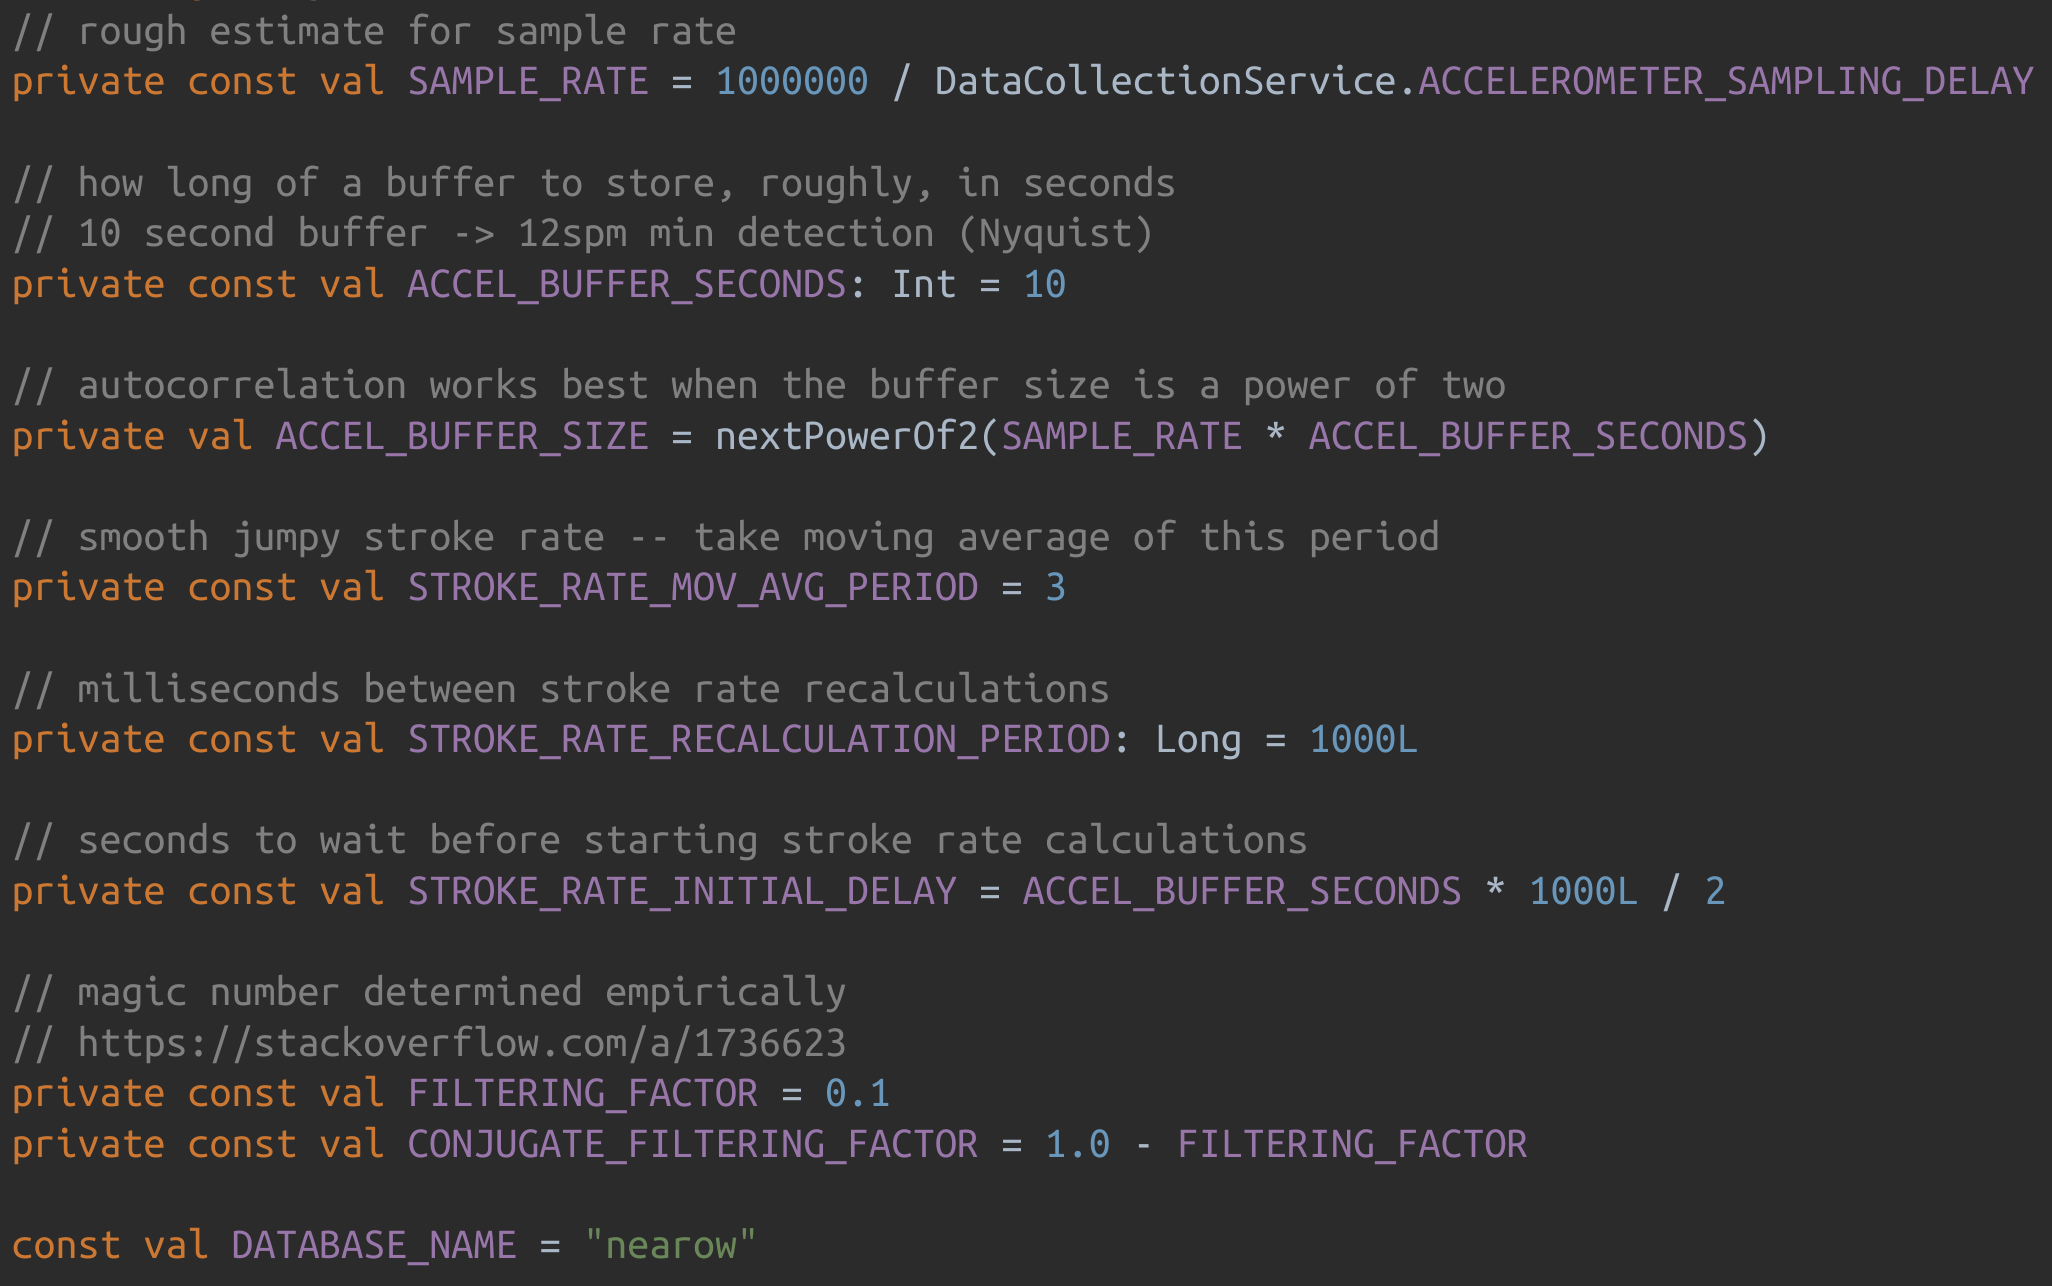
\includegraphics[width=1.0\textwidth]{code-dataProcessor-companion.png}
  \caption{}
  \label{fig:companionDataProcessor}
\end{figure}

Figure \ref{fig:companionDataProcessor} show the various configurable compile-time constants are configurable. In theory these could be exposed to the user, but the average rower has no need to configure any of the parameters shown. Most of these numbers were either determined empirically through testing or by calculation.

Let me draw your attention to the \texttt{ACCEL\_BUFFER\_SECONDS} quantity that specifies how large of a buffer to store with acceleration readings. This was chosen to be $10$\si{\second}. By Nyquist's theorem, frequencies with a wavelength of up to $5$\si{\second} can be detected. That results in a $60 \div 5 = 12$~spm minimum detection frequency. Stroke rates lower than $12$ are incredibly rare and inefficient. Perhaps only in the case of a specific drill might the stroke rate drop that low. A typical paddling stroke rate could go as low as $15$, which makes $12$ a reasonable lower bound.

\begin{figure}[h!]
  \centering
  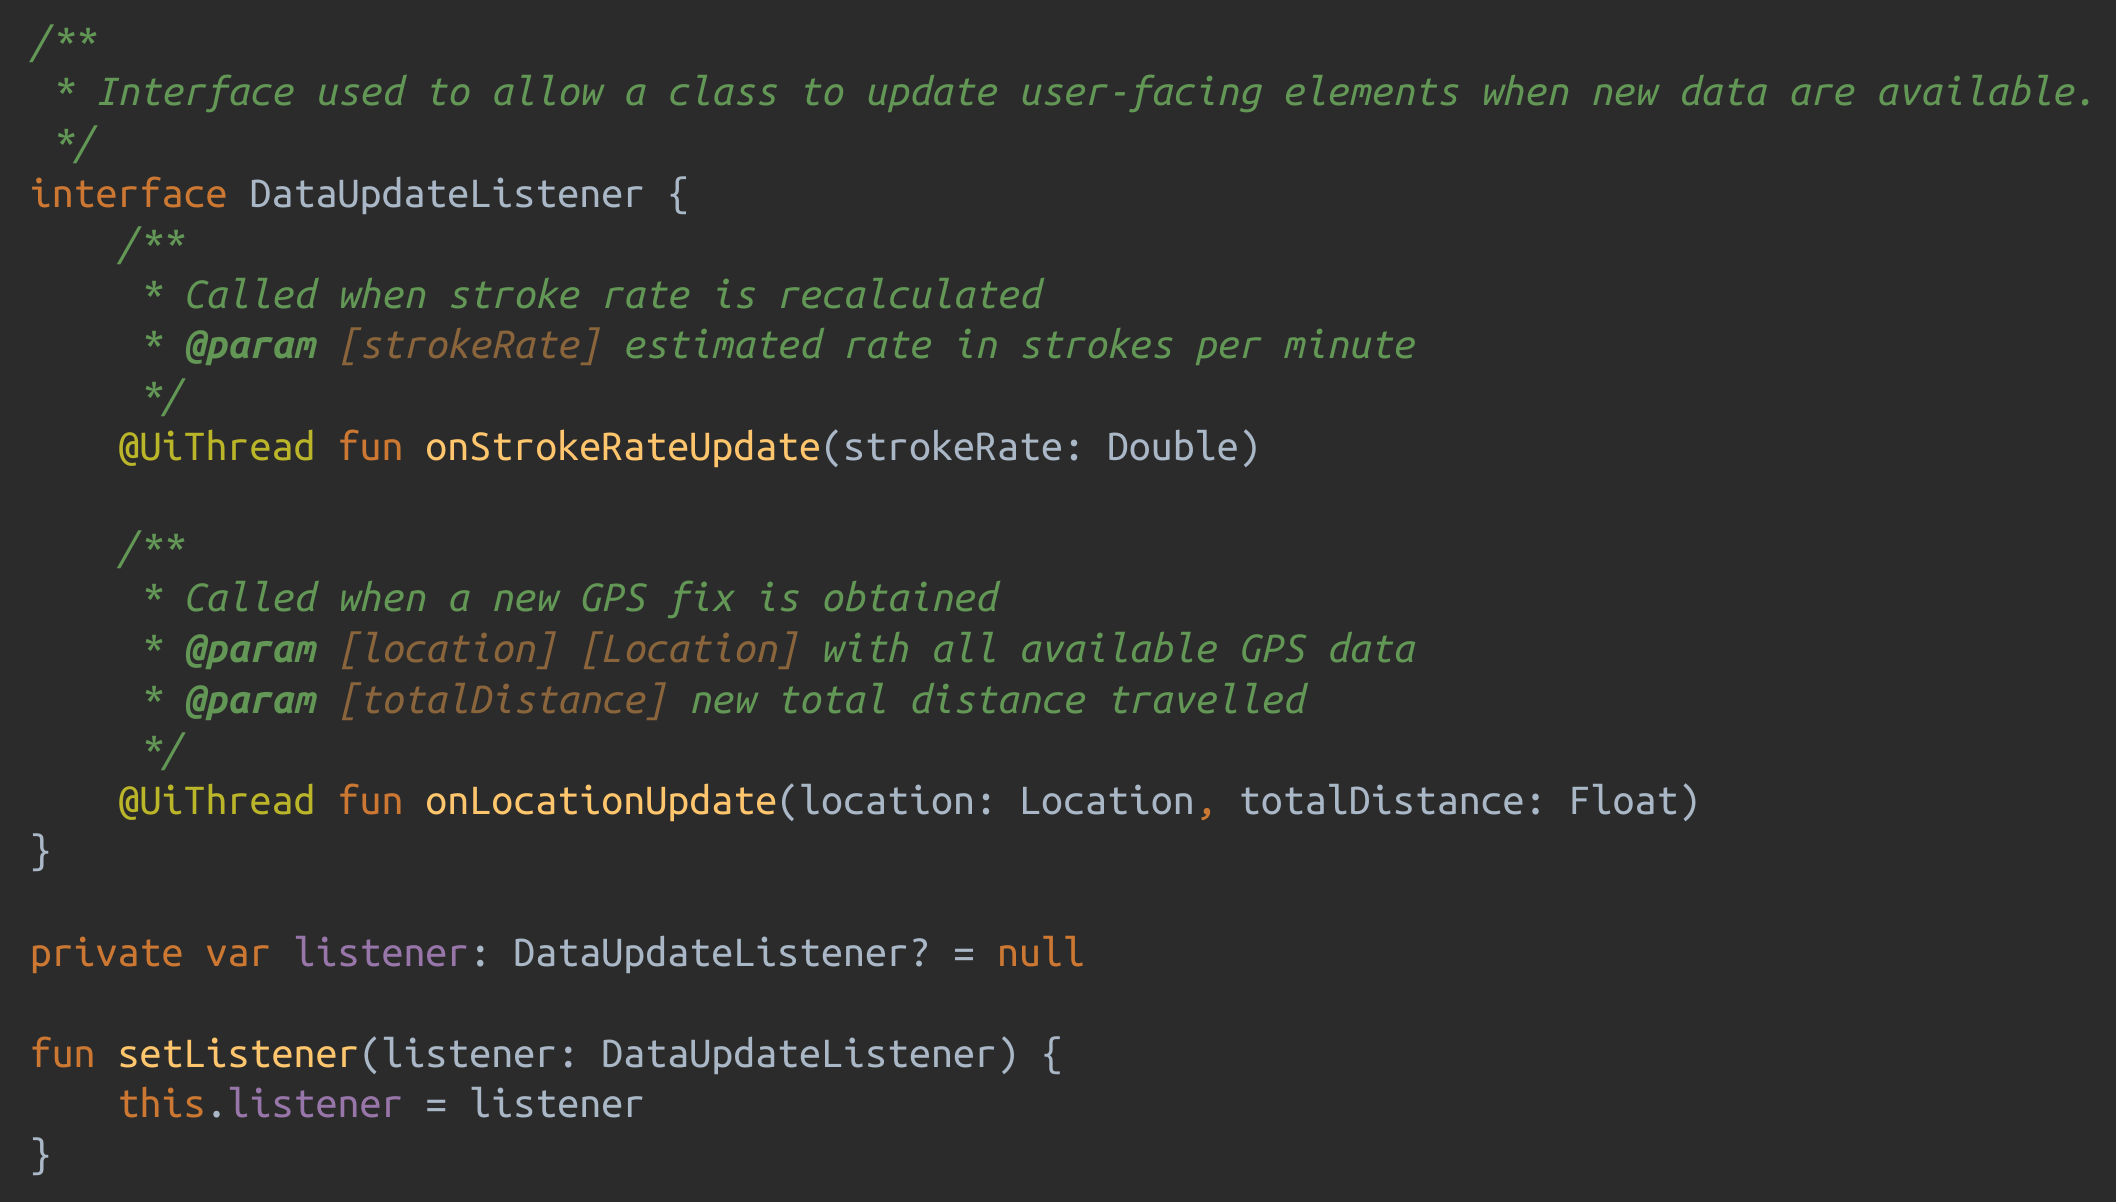
\includegraphics[width=1.0\textwidth]{code-dataProcessor-DataUpdateListener.png}
  \caption{}
  \label{fig:DataUpdateListener}
\end{figure}

The \texttt{DataProcessor} provides an \texttt{interface} that allows a UI class to listen for updates to the stroke rate or location and appropriately update the user interface. The \texttt{DataUpdateListener} interface is defined within the \texttt{DataProcessor} class, as shown in figure \ref{fig:DataUpdateListener}. The methods of the \texttt{DataUpdateListener} interface are marked with the \texttt{@UiThread} annotation so that a error message is logged if they are called from a non-UI thread.

\section{Data storage}

\section{File export}

\section{User interface}

\printbibliography[heading=bibintoc]

\end{document}
